% interactcadsample.tex
% v1.03 - April 2017

\documentclass[]{interact}

\usepackage{epstopdf}% To incorporate .eps illustrations using PDFLaTeX, etc.
\usepackage{subfigure}% Support for small, `sub' figures and tables
%\usepackage[nolists,tablesfirst]{endfloat}% To `separate' figures and tables from text if required

\usepackage{natbib}% Citation support using natbib.sty
\bibpunct[, ]{(}{)}{;}{a}{}{,}% Citation support using natbib.sty
\renewcommand\bibfont{\fontsize{10}{12}\selectfont}% Bibliography support using natbib.sty

\theoremstyle{plain}% Theorem-like structures provided by amsthm.sty
\newtheorem{theorem}{Theorem}[section]
\newtheorem{lemma}[theorem]{Lemma}
\newtheorem{corollary}[theorem]{Corollary}
\newtheorem{proposition}[theorem]{Proposition}

\theoremstyle{definition}
\newtheorem{definition}[theorem]{Definition}
\newtheorem{example}[theorem]{Example}

\theoremstyle{remark}
\newtheorem{remark}{Remark}
\newtheorem{notation}{Notation}


% tightlist command for lists without linebreak
\providecommand{\tightlist}{%
  \setlength{\itemsep}{0pt}\setlength{\parskip}{0pt}}



\usepackage{hyperref}
\usepackage[utf8]{inputenc}
\def\tightlist{}
\def\UrlBreaks{\do\/\do-\do?}

\usepackage{booktabs}
\usepackage{longtable}
\usepackage{array}
\usepackage{multirow}
\usepackage{wrapfig}
\usepackage{float}
\usepackage{colortbl}
\usepackage{pdflscape}
\usepackage{tabu}
\usepackage{threeparttable}
\usepackage{threeparttablex}
\usepackage[normalem]{ulem}
\usepackage{makecell}
\usepackage{xcolor}

\begin{document}


\articletype{}

\title{Material Culture Networks in Tonto Basin}


\author{\name{Robert J. Bischoff$^{a}$}
\affil{$^{a}$School of Human Evolution and Social Change, Arizona State
University, Tempe, AZ}
}

\thanks{CONTACT Robert J.
Bischoff. Email: \href{mailto:rbischoff@asu.edu}{\nolinkurl{rbischoff@asu.edu}}}

\maketitle

\begin{abstract}
Network analysis has a strong foundation in Southwest archaeology, yet
the combination of multiple types of artifacts in one
analysis--multilayer network analysis--has not been formally applied
except within a single artifact type. Many studies consider material
culture holistically, yet network analysis has the advantage of focusing
specifically on the relationships between entities (often communities)
and how the structure of a network can benefit particular entities. This
study takes architecture, ceramic, projectile point, and site location
data from the Roosevelt Platform Mound Study and combines these data
into a multilayer network analysis. This analysis provides a way to test
the co-variance of these types of material culture with each other and
with spatial variation. The results demonstrate a strong association
between projectile points and spatial distance. Sites containing
roomblock architecture are highly central in the ceramic network but
have low centrality in the projectile point network. Overall, the
ceramic and projectile point networks exhibit significant differences.
This indicates that the social networks that created these patterns had
different social mechanisms. One potential cause of these differences is
gendered spheres of interaction with men exchanging projectile points
and women exchanging ceramics.
\end{abstract}

\begin{keywords}
American Southwest; network analysis; multilayer networks; Hohokam;
projectile points; ceramics; computational archaeology; gender
\end{keywords}

\hypertarget{introduction}{%
\section*{Introduction}\label{introduction}}
\addcontentsline{toc}{section}{Introduction}

Network science has many applications for archaeologists. It can be
particularly useful for breaking out of traditional spatial categories
and examining data through new lenses
\citep{Feinman2020-nf, Holland-Lulewicz2021-eb}. Multilayer network
analysis combines multiple networks into one analytical framework
\citep{Kivela2014-mh}. Social systems are complex webs of
interrelations. There is too much involved to model the material culture
of even a technologically simple society. But certainly analyzing more
than one type of material culture provides a more complete understanding
of the social dynamics involved in the networks of interaction we wish
to understand. Yet, there are few examples of multilayer networks in
archaeology \citep{Giomi2022-dn, Upton2019-yg} and none I am aware of
that extend beyond ceramics.

Network studies are particularly prominent in the Southwest and there
are examples of network studies that consider multiple types of material
culture. For example, Mills and colleagues \citeyearpar{Mills2013-gc}
used ceramics and obsidian to understand the transformation of large
scale social networks. Peeples \citeyearpar{Peeples2018-ib} used
ceramics and architecture to understand identity and social change in
the Cibola region. This paper is an application of multilayer network
analysis that seeks to further network research by examining multiple
types of material culture in one framework. Given the frequent focus on
single types of artifacts in network research, a primary question I seek
to address is whether networks based on different types of material
culture are positively correlated. This is an important question because
archaeologists often make inferences based solely on ceramics or other
types of material culture. Evidence regarding the ways material culture
co-vary will help archaeologists direct future research. Furthermore, I
also seek causal explanations for the co-variance, or lack thereof, for
material culture in the case study I present here.

Tonto Basin holds great potential for archaeological research due to the
large cultural resource management projects conducted in the region
primarily in the 1980s-1990s
\citep{Ahlstrom1991-eb, Ciolek-Torrello1994-ds, Doelle1992-lu, Rice1998-ku},
as well as the large number of syntheses and other studies focusing on
the area
\citep[e.g.,][]{Clark2004-uw, Dean2000-uc, Elson1995-tb, Elson2000-zq, Hill2015-at, Huntley2016-em, Lange1992-gp, Lyons2003-yy, Lyons2006-to, Lyons2012-pr, Neuzil2008-zd, Oliver2001-tu, Stark1998-mu, Watts2013-ub}.
This analysis uses data from the Roosevelt Platform Mounds Study (RPMS),
the largest of these projects \citep{Rice1998-ku}, to examine basic
architectural data, typed ceramics, and a recent projectile point
analysis \citep{Bischoff2022-rg}. There are two null hypotheses tested
in this analysis: (1) that the data is spatially correlated--meaning
that sites nearest to each other will be most alike--and (2) that the
architecture, ceramics, and projectile points will all be positively
correlated--meaning that similar types of architecture, ceramics, and
projectile points will be found at the same sites. In reality, I
expected significant variation between these types of material culture.
As will be demonstrated, the results indicate a positive correlation
between projectile point similarity and spatial distance. Furthermore,
ceramic and projectile point networks (hereafter point networks) exhibit
significant differences. I posit that the differences in these networks
are connected to the identities of the individuals creating the original
social networks: particularly that of gender.

\hypertarget{tonto-basin}{%
\subsection{Tonto Basin}\label{tonto-basin}}

Tonto Basin is located in east-central Arizona and features Tonto Creek
flowing from the Mogollon Rim into the Salt River (figure 1). Parts of
the region have been intensively studied, while certain time periods and
much of the uplands have been less intensively sampled \citep[see][ for
a recent overview]{Clark2021-lu}. The basin was also conveniently
located along regional travel routes, allowing major
settlements--particularly those with platform mounds--to participate and
benefit from this exchange
\citep[p.~129-133]{Caseldine2022-uu, Wood2000-ze}. The junction of the
Salt River and Tonto Creek now forms Roosevelt Lake since the damming of
the confluence of the Salt River and Tonto Creek. It was the expansion
of the dam that precipitated the RPMS and its related projects in the
late 1980s-1990s. Some important regional differences may have
differentiated sites along the Salt River and Tonto Creek arms of
Roosevelt Lake \citep{Lyons2013-ya, Simon2001-am} based on non-local
ceramics and obsidian. All of the artifacts/data from the RPMS project
are hosted at the Center for Archaeology and Society at Arizona State
University, and the data in this study come exclusively from this
project.

\begin{figure}
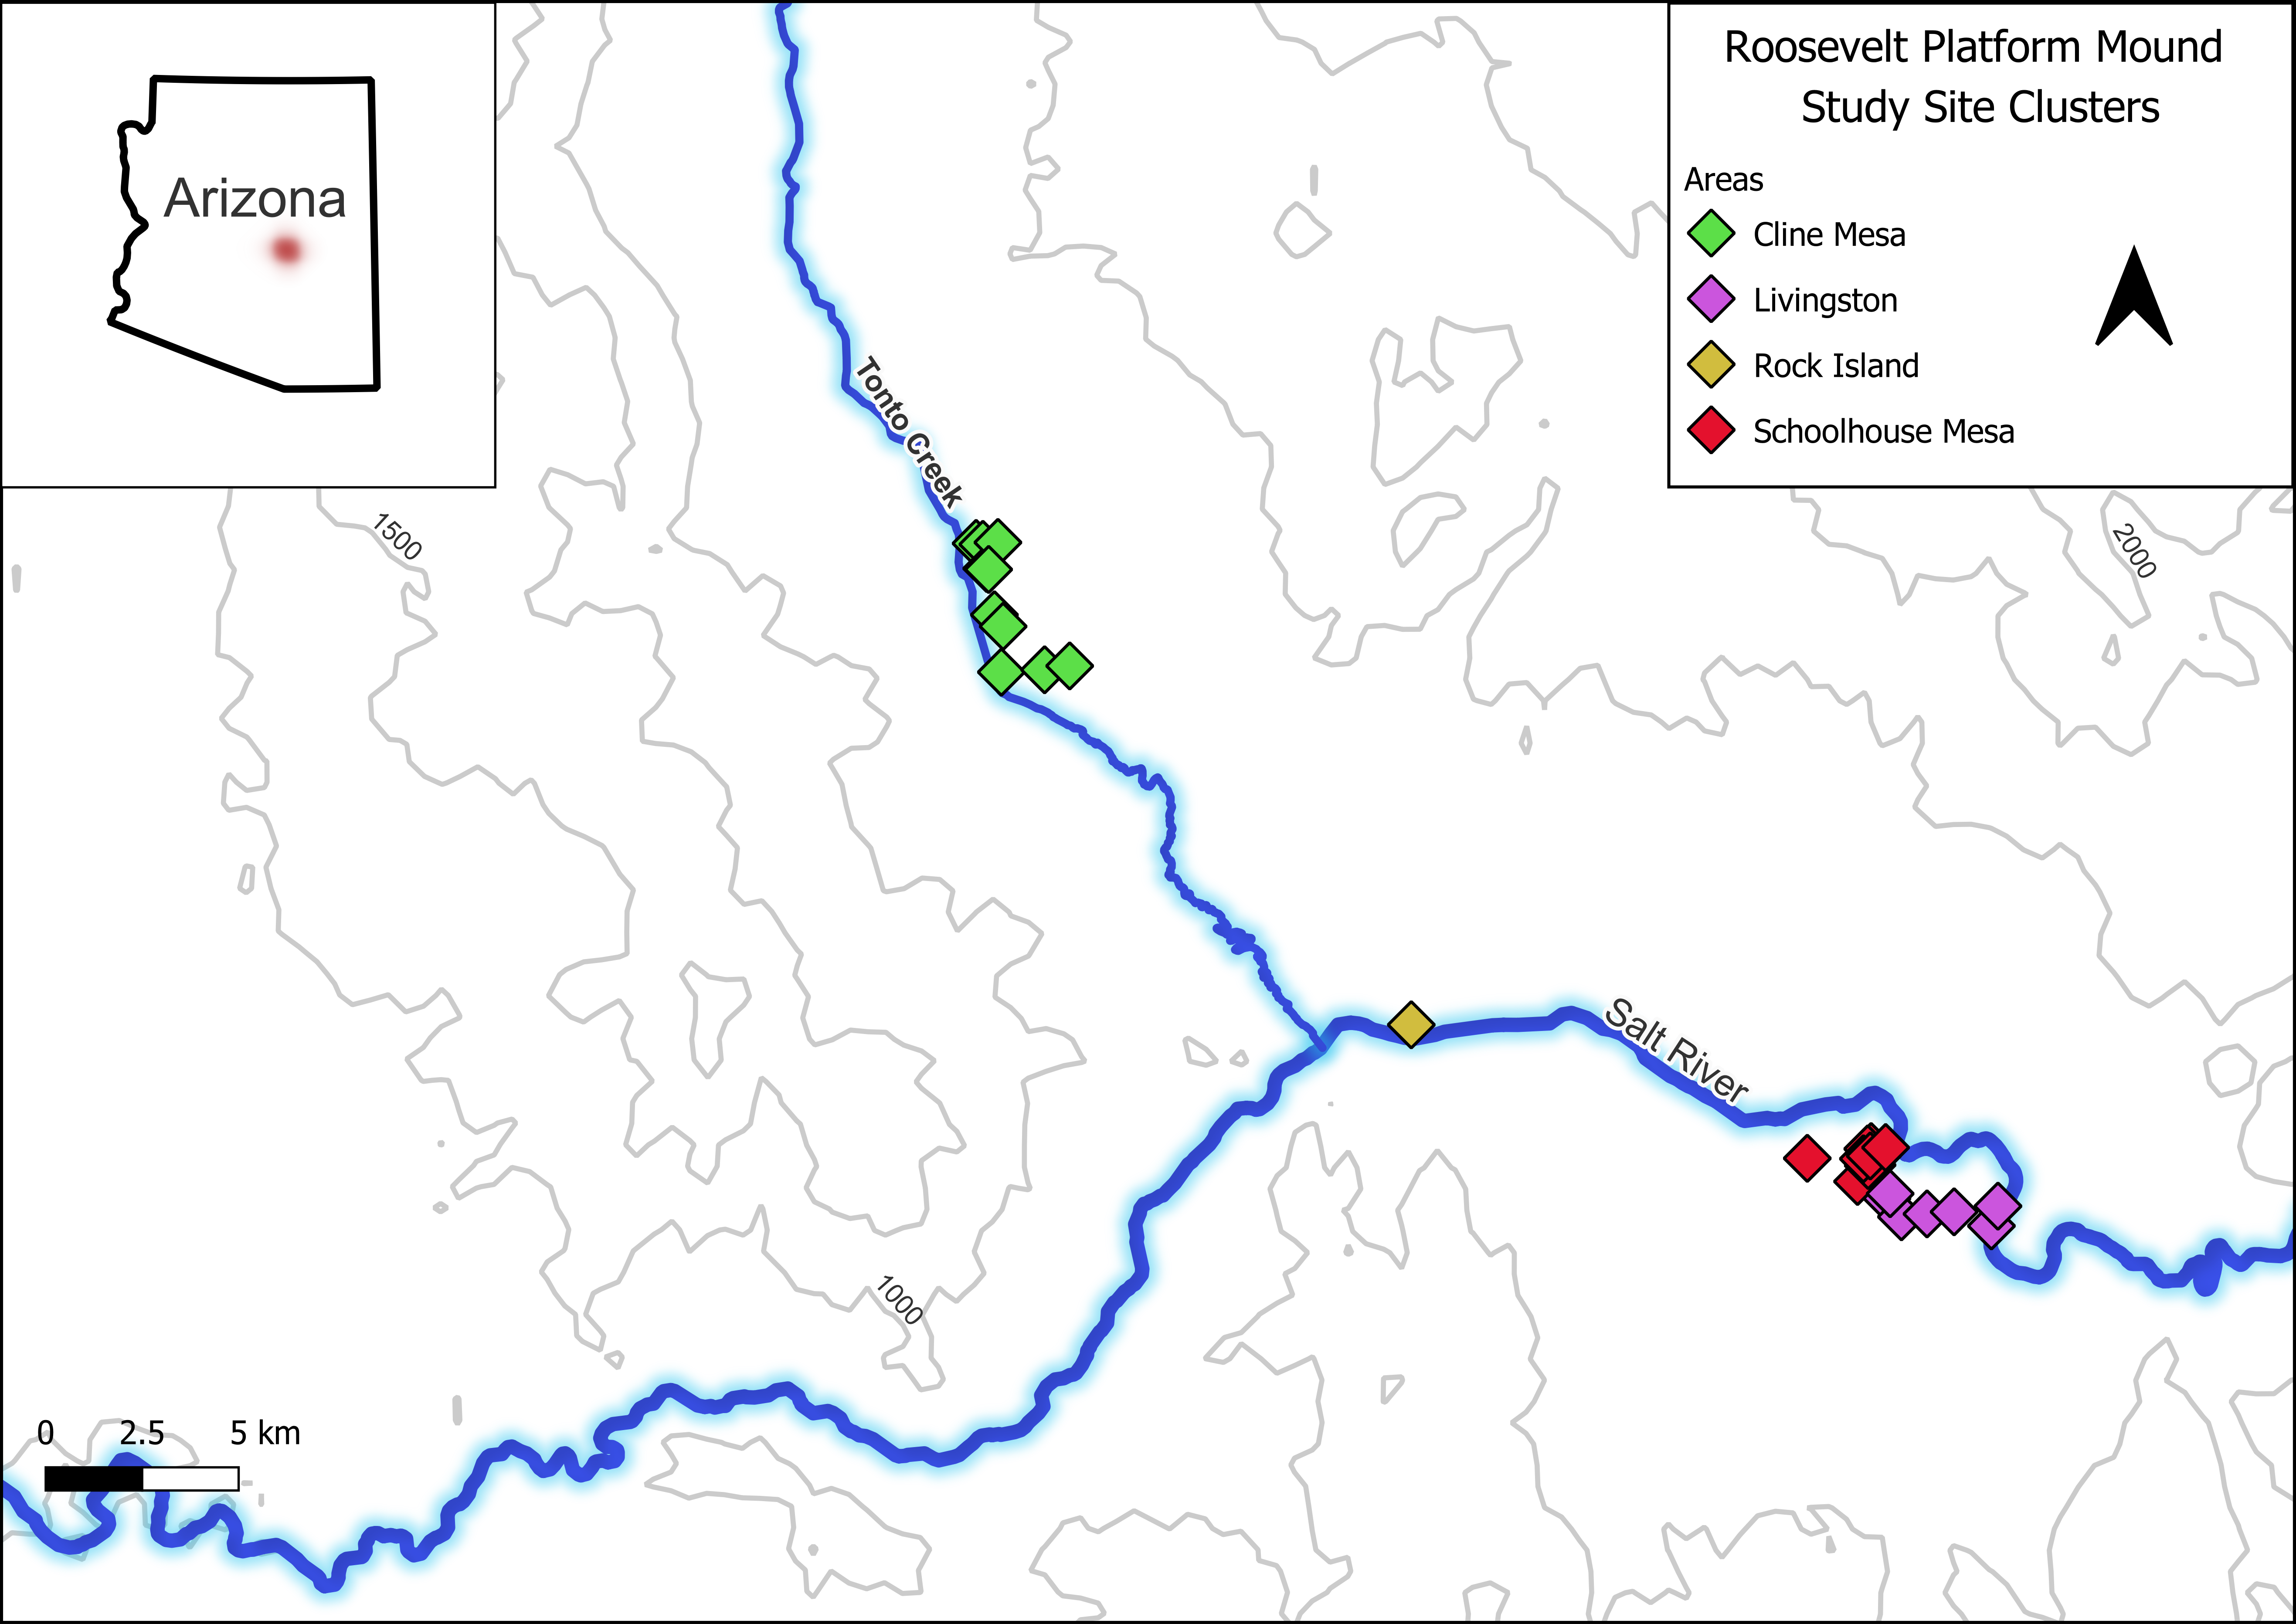
\includegraphics[width=1\linewidth]{figures/TontoBasinSitesv3} \caption{Map of archaeology sites from the Roosevelt Platform Mounds Study in Tonto Basin. Groups use the original assignments.}\label{fig:TontoBasinSites}
\end{figure}

Tonto Basin was occupied, although likely not continuously, from the
Archaic through the late Classic period. The height of occupation,
particularly the sites excavated during the project, dates between AD
1275 and 1325, which corresponds to the Roosevelt Phase. The Roosevelt
phase is notable for the appearance of Salado pottery and platform
mounds--probably introduced from the Phoenix Basin \citep{Elson1996-ym}.
Moderate occupation continued into the Gila phase (AD 1325-1450), which
was characterized by population loss and aggregation into larger sites.
This phase marks the end of recognizable occupation in the area until
the historic period.

One aspect of Tonto Basin that has caught the attention of researchers
is its location in a border zone between the Hohokam, Mogollon, and
Ancestral Pueblo regions
\citep[e.g.,][]{Caseldine2022-uu, Clark2001-ck, Elson1994-hk, Hill2015-at, Huntley2016-em, Lyons2012-pr, Lyons2013-ya, Neuzil2008-zd, Wood2000-ze}.
Of particular note is the presence of masonry roomblock architecture and
pottery uncharacteristic of the local Hohokam traditions, which has been
interpreted as Kayenta immigration into Tonto Basin
\citep{Clark2001-ck, Lyons2003-yy, Lyons2006-to, Stark1998-mu}. This
migration into the Tonto Basinwas part of a larger migration from north
to south and is associated with the origin of the Salado phenomenon.
Salado pottery production was widespread across southern Arizona, but
often the largest sources of production was centered at the location of
a former Kayenta enclave
\citep{Hill2015-at, Huntley2016-em, Lyons2012-pr, Neuzil2008-zd}. The
connection between immigration and an important type of decorated
pottery in the region suggests that sites with roomblocks may have
higher centrality in ceramic networks. Having high centrality means they
have more connections to other nodes (i.e., sites). The presence of
migrant communities in Tonto Basin invites questions regarding the
relationship between sites--particularly between migrant and local
communities. A network approach is an ideal way to examine the
relationships between sites. Evidence that projectile points move
between sites \citep[e.g.,][]{Watts2013-ub} indicates that this is also
a productive line of analysis, and one that is less-commonly pursued
compared to architecture and ceramics.

\hypertarget{network-analysis}{%
\section*{Network Analysis}\label{network-analysis}}
\addcontentsline{toc}{section}{Network Analysis}

Network analysis is a flexible tool for analyzing many types of data
\citep[see][]{Brughmans2023-uj}. The key element is that some way must
be determined to tie each entity together. This analysis uses sites as
nodes in the network and some type of similarity as a tie to connect
each node. Each type of similarity depends on the type of data. Table 1
lists the 11 sites with sufficient data to include in this study with
the types of architecture present, periods occupied, and total number of
ceramics and complete projectile points found at each site. The lack of
complete projectile points at some sites is the largest caveat in this
study, but complete points were necessary for the type of projectile
point analysis used. The periods, architecture types, and ceramic types
were assigned during the RPMS project and can be found in the project
reports \citep{Rice1998-ku}. This is not a random sample of Tonto Basin
sites. It is merely a sample of convenience. Sampling can have a major
impact on conclusions. In this case, I am not drawing conclusions based
on a complete network or the existence of a random sample (though biases
can still affect the results). Rather, I am interested in whether the
types of material culture present in this study co-vary with each other
and with space. These questions do not require a complete network.

\hypertarget{defining-networks-and-relations}{%
\subsection{Defining Networks and
Relations}\label{defining-networks-and-relations}}

Network approaches are best suited where the relationships between
entities are of primary interest. In this case, the entities are defined
as archaeology sites. The archaeology sites in turn represent a group of
individuals who lived or visited the area of the site and left material
remains behind. Ideally, studying social relations would be approached
at the individual level, but rarely can archaeologists address
archaeological data with that level of specificity. Watts
\citeyearpar{Watts2013-ub} used projectile points from Tonto Basin in
just such a study. His analysis of flake scar patterning identified
individual knappers, or at least clusters of knappers with similar
knapping styles, and the distribution of their projectile points around
Tonto Basin. He found strong connections between many parts of the
eastern Tonto Basin. Unfortunately, this study will only attempt a
site-level analysis. Watt's study does, however, illustrate how
relations can be defined between nodes in a network analysis. He used
similarity networks where the points that had similar flaking styles
were connected together. Similarity networks are a commonly used type of
network in archaeology
\citep[e.g.,][]{Birch2018-xx, Borck2015-jy, Cochrane2010-oa, Golitko2015-we, Lulewicz2019-lu, Mills2013-wq, Peeples2018-ib, Terrell2010-hd}.
These studies use a variety of artifacts and methods to construct their
networks, but each has demonstrated the utility of network methods
within archaeological contexts. This study also uses similarity networks
to group sites by similarity in ceramic assemblages and similarity in
projectile point forms.

Yet, it can be difficult to understand how a similarity network is
related to a past social network. What kinds of interactions are
represented by similarities in projectile points or in ceramics?
Answering this question is also a crucial step in interpreting networks.
One way to examine relations between individuals who make or use similar
types of projectile points or pots is to talk about identity. Identity
can be a troubling topic for anthropologists. There are numerous
meanings given to it and numerous scales at which it applies
\citep{Brubaker2000-na}, but Peeples \citeyearpar{Peeples2018-ib} has
introduced archaeologists to a more practical approach that is useful
here. This approach views identity as existing along two axes: one
categorical and the other relational. Relational identification is the
process of identifying with someone due to frequent interaction.
Categorical identification is the process of identifying with someone
because you belong to a recognized social group. For example, members of
the same moiety would share a categorical identity. They would likely
also share a relational identity if they frequently interacted. These
identities can be reflected in material culture. Pottery makes a good
example. Peeples \citeyearpar[p.~151]{Peeples2018-ib} notes that bowls
in the Cibola region were sometimes painted with a bright, red slip with
designs painted on the interior and they were among the first in the
Southwest to have designs on the exterior. This is a strong indication
of categorical identity. The potters were attempting to make a clear
signal for whoever saw the pot. Relational identity can be seen in the
way the potter prepares the clay recipe and smooths the coils. The
particulars of these actions would be learned from close interaction
with a teacher or other potters. In this way, relational identity can be
compared to communities of practice \citep{Lave1991-ik, Wenger1998-rx}.

In this analysis, I argue that ceramics and architecture are more likely
to represent categorical identity. The architecture discussed is highly
visible and representative of historical group membership. The ceramics
are grouped into types based primarily on decoration, which is strongly
indicative of group membership. What this means is that links between
nodes in the cer The details of architecture and ceramics used in this
study are discussed in a future section, but it is important to note
that these designations as categorical or relational are contextually
dependent on this study. Clark \citeyearpar{Clark2001-ck} has an
excellent discussion on material culture and its relationship to
identity. He identifies certain patterns, but his synthesis and other
research
\citep{Carr1995-mq, Carr1995-sh, Dietler1998-zo, Gosselain1998-qd, Gosselain2000-wf, Gosselain2016-as, Hodder1982-no, Huntley2008-qu, Lemonnier1986-le, Lyons2003-yy, Neuzil2008-zd, Sassman2001-sw, Stark1998-mu, Wiessner1983-ei, Wiessner1997-su}
strongly indicates that the relationship between material culture and
identity is culturally relative. Projectile points can in some cases
indicate group membership \citep{Wiessner1983-ei, Wiessner1997-su}, but
in this case the triangular and side-notched points were likely used for
different purposes \citep[see][]{Loendorf2015-ww, Sliva2002-oz}. Styles
were difficult to determine for the original researchers
\citep{Rice1994-rk}, and I had the same difficulty. In my opinion, the
subtle differences between projectile point outlines are more
representative of interactions between knappers than markers of group
identity for this particular case. This is indicative of relational
identity. There are no environmental reasons to assume differences in
projectile points, as each site was in a similar ecozone. Each hunter
would have been using the points for the same game and differences in
point styles would have been primarily cultural \citep{Sliva2002-oz}.

There is one other aspect to these relations that I believe played an
important role. A central way people identify themselves is by gender.
Gender roles, like identity, can also vary in complex ways, but for the
purposes of this analysis I will use a simplified model. Women made
pottery and men made projectile points. This was not always true of
course, but this fits the available data for the Hohokam
\citep[p.~253]{Crown1996-xb, VanPool2010-im}. An examination of the
burial record for the RPMS study shows no obvious indication that women
made pottery, only that both men and women were buried with pottery
\citep[Table 10.7]{Loendorf1998-ln}. On the other hand, projectile
points were almost exclusively buried with males. This does not mean
that a man could not move pots from one site to another or that a woman
could not do the same with a projectile point, but, in general,
differences in point and ceramic networks are most likely to indicate
differences in gender networks.

From this discussion, I expect the ceramic and point networks to differ
in two ways. I expect the ceramic network to represent categorical
identity among women, and I expect the point network to represent
relational identity among men. This makes the networks somewhat more
difficult to compare. Ideally, we would have networks of the same
identity type, but it does provide the expectation that we should see
significant differences in the networks.

The network for architecture, ceramics, and projectile points, were
created using the Jaccard similarity coefficient \citep{Jaccard1912-na}
to determine the links between each site. This is a simple measure of
similarity that does not take into account abundance. It was chosen due
to the large differences in sample sizes between sites for the ceramics
and projectile points and because count data were irrelevant or not
readily available for the architectural data.

\begin{table}

\caption{\label{tab:sites}Project Sites and Data}
\centering
\resizebox{\linewidth}{!}{
\begin{tabular}[t]{llllrr}
\toprule
Site & Area & Architecture & Phase & Ceramics & Points\\
\midrule
AZ U:3:128 (ASM) & Cline Mesa & compound & Roosevelt, Gila & 7,522 & 5\\
AZ U:4:032 (ASM) & Cline Mesa & compound & Sacaton, Roosevelt & 5,352 & 3\\
AZ V:5:119 (ASM) & Livingston & compound & Roosevelt & 1,679 & 3\\
Bass Point Mound & Rock Island & platform mound & Roosevelt & 27,602 & 13\\
Cline Terrace Mound, Monster Ruin & Cline Mesa & platform mound & Roosevelt, Gila & 169,567 & 45\\
\addlinespace
Indian Point Complex & Cline Mesa & compound, roomblock & Roosevelt, Gila & 39,493 & 14\\
Pinto Point Mound & Livingston & compound, platform mound & Roosevelt & 19,174 & 21\\
Saguaro Muerto & Livingston & roomblock & Roosevelt & 13,458 & 5\\
Sand Dune Site & Livingston & compound & Roosevelt & 10,545 & 12\\
Schoolhouse Point Mesa Complex & Schoolhouse Mesa & compound & Roosevelt & 74,592 & 12\\
\addlinespace
Schoolhouse Point Mound & Schoolhouse Mesa & platform mound & Roosevelt, Gila & 240,635 & 36\\
\bottomrule
\end{tabular}}
\end{table}

The types of similarity used in this study are varied depending on the
type of network. Part of this analysis is a visual approach and some of
the methods require non-weighted links, thus I will be only using the
strongest links. There is rarely a clear dividing line between similar
and not similar. This can be a challenge for network analysis, because
we can end up with networks where every node is connected to every other
node. The decision to binarize a network--remove the weakest links and
then consider each link of equal value--has its drawbacks
\citep{Peeples2013-tj}, but is necessary in this case. A solution is to
assign weights to each link that defines the strength of the tie. These
networks are often difficult to visualize, and some network algorithms
do not allow for weights. A common approach is to keep only the
strongest ties by either ranking the ties or using a cutoff value.

I used ranked links to keep consistent values between networks. This
involved calculating the strength of similarity between each site in the
network and then ranking the strength of similarity. The top \textbf{n}
connections between each site were kept and the rest were discarded. In
practice, not every node will have the same number of connections. Some
may have fewer ties if there are not enough nodes that are similar. More
ties can exist when there are ties in the ranks. Because the network is
not directed (meaning the ties indicate similarity in both directions)
one node can have several ties pointing to it because that node was in
the top \textbf{n} of multiple other nodes. In the latter case, this is
a good indication of a central node in the network. Because I am using
several types of networks, there is no common cutoff value I can use for
the number of ties to keep. Instead of arbitrarily picking one value, I
have calculated each metric using networks composed of the top 3-10
ties. Meaning that each metric is calculated for a network composed of
ties with the top 3 connections, and the process is repeated for new
networks composed of ties with the top 4 connections, and so forth.
Examining the range of these metrics provides a more robust analysis.

Two network metrics are discussed in this analysis: eigenvector
centrality and multilayer network correlation--the second will be
discussed in the next section. Node centrality is a common way to
quantify networks \citep{Borgatti2005-iz}. Centrality is a measure of
the influence of the node on the network. Nodes with higher centrality
generally derive or generate greater benefits from the network. For
example, if I have many friends, then I can call in more favors.
Eigenvector centrality is one way to measure node centrality and is
commonly used in archaeology. This metric describes how well a node is
connected to the network as a whole and is helpful in comparing
different networks containing the same nodes. For example, if my friends
have many friends, then I will have a greater advantage then someone
with an equal number of friends, but whose friends have few friends.
Essentially, this is a way of measuring second-order and beyond
connections. Eigenvector centrality is also more robust to missing nodes
than other measures \citep{Peeples2017-kl}, a major problem in most
archaeological studies.

A single network is typically used in network analyses, but multilayer
networks can be more informative. Multilayer networks are layered
networks where nodes have different types of connections
\citep{Kivela2014-mh}. In this analysis, each network has the same
nodes--each archaeological site--but different types of relationships
between them. The combination of these individual networks is a
multilayer network (also called a multiplex network). Multilayer
networks allow for methods to be applied on multiple networks at once
\citep[see][]{Brodka2018-vz}. The method applicable to this analysis is
layer correlation. Either Pearson or Spearman rank correlation can be
computed to determine the strength and direction of correlation between
each layer. Bródka and colleagues \citeyearpar{Brodka2018-vz} have
provided an R package to compute these statistics, which I have used in
this study. They recommend the Pearson correlation in most
circumstances. I will display the results of the Pearson correlation,
but the Spearman correlation provided similar results. Eigenvector
centrality was mentioned in the previous section, but it is also
calculated as a multilayer eigenvector centrality. In this case the
centrality measure is simply the mean of the eigenvector centraliy for
each separate layer, as the layers are not interdependent
\citep{Frost2022-lr}. Multilayer eigenvector centrality results are only
presented for the combination of ceramic and point layers. These
networks can be thought of as dependent variables for the spatial and
architectural networks--meaning spatial distance and architecture are
considered to be important variables determining the structure of the
ceramic and point networks.

The robustness of results were tested by randomly sampling the
underlying network matrices 10,000 times and comparing the results to
the random samples to obtain a p-value. This provides a baseline that
determines how likely it is to obtain a given result by chance.

Certain caveats must be acknowledged. All archaeologists deal with
missing data, which can greatly affect the results of analysis. Network
analysts have grappled with this question and often use resampling or
similar methods to deal with this problem
\citep{Bischoff2021-sf, Bolland1988-zm, Borgatti2006-jl, Brughmans2023-uj, Costenbader2003-st, Galaskiewicz1991-qb, Gjesfjeld2015-hw, Lee2009-wr, Rivera-Hutinel2012-ik}.
Regardless of statistical methods, unaccounted for biases will still
produce invalid results \citep{Bischoff2021-sf}. The most important bias
that may affect these findings is chronology. For example, Bass Point
Mound and Cline Terrace Mound were probably not occupied at the same
time \citep{Jacobs1997-ob, Lindauer1995-wq}. Does that invalidate the
network analysis? I do not think so. While the networks involve nodes as
sites, what the networks are really meant to represent are groups of
people. Furthermore, they are not individuals, but the aggregate
decisions of people over more than one generation. Current models of
Hohokam social groups suggest a certain residential stability
\citep[p.~336]{Craig2017-rg}. Perhaps the residents of these sites were
not physically located at the site at the same time as the other
inhabitants were located at their site, but they may have been at
another nearby location. The spacing of settlements may indicate a
corporate form of social organization
\citep[p.96]{Clark2004-uw, Rice1998-rz}. If this is accurate, then the
communities inhabiting the sites may likely have existed in some form
prior to the establishment of any particular site and have continued on.
It is these communities that the network analysis is attempting to
capture. Still, evidence indicates that most sites were contemporaneous.
For example, Cline Terrace Mound and Schoolhouse Point were most
probably occupied at the same time \citep{Lyons2013-ya}. It is best,
though, to think of these interpretations as estimations based on
incomplete data.

\hypertarget{spatial}{%
\subsection*{Spatial}\label{spatial}}
\addcontentsline{toc}{subsection}{Spatial}

The simplest network is the spatial network. This network was created by
calculating the Euclidean distance from every site to every other site.
Euclidean distance is a shortcut that does not represent actual travel
routes. Least cost paths provide more accurate data \citep[see][ for an
application in Tonto Basin]{Caseldine2022-uu}, yet an analysis in
similar terrain indicates that for distances longer than those in this
study the benefits of least cost path distances in place of Euclidean
distance are negligible \citep{Bischoff2017-gx}. Least cost paths are
also hampered by the presence of Roosevelt Lake and other modern impacts
on the landscape. The spatial network created here is equivalent to
proximal point analysis, which was used in one of the earliest network
studies in archaeology \citep{Terrell1977-co} and continues to be used
to study potential pathways of interaction
\citep[see][]{Broodbank2000-pg, Collar2013-fb}. The inclusion of a
spatial network serves as a null hypothesis to test the other networks
against.

\hypertarget{architecture}{%
\subsection*{Architecture}\label{architecture}}
\addcontentsline{toc}{subsection}{Architecture}

The architectural components consisted of compounds, roomblocks, and
platform mounds. Compounds were the typical residential structures in
the area and featured multiple houses built from masonry and/or adobe
around a courtyard. Platform mounds were formed from large masonry and
adobe retaining walls with a cell-like interior filled with trash and
rubble. They were common in the Hohokam region throughout the Classic
period. Some sites had pit houses from earlier occupations, but most
excavation was focused on the Roosevelt and Gila phases so these few pit
houses were removed from the analysis \citep[see][]{Rice1998-ku}. Each
site was classified as a platform mound if one was present regardless of
other architecture or as a roomblock if a platform mound was not present
regardless of other architecture. Thus, if a site is labeled a platform
mound it may have other architecture. Sites were thus labeled to
emphasize the most distinctive form of architecture, but all types of
architecture were present in the analysis, and all architectural
features included in the analysis can be seen in Table 1.

\hypertarget{ceramics}{%
\subsection*{Ceramics}\label{ceramics}}
\addcontentsline{toc}{subsection}{Ceramics}

The ceramic network consists of 55 types--plainware and
decorated--ranging from 181,666 Plain Brown Ware sherds to a single
Black Mesa Black-on-white sherd. A single sherd is not much, but it is
still indicative of trade or movement. The median sherd count was 157
for all types. The ceramic data was accessed from the cyberSW database
\citep{Mills2020-tb}, which keeps the full citations for the ceramic
data. The standard caveats for ceramic analysis apply to this analysis
as well: problems with sherd misidentification and data errors.

\hypertarget{projectile-points}{%
\subsection*{Projectile Points}\label{projectile-points}}
\addcontentsline{toc}{subsection}{Projectile Points}

The ceramic and architectural data are available in suitable formats for
analysis, but the original projectile point analysis was too general for
the purposes of this study \citep[see][ for details]{Rice1994-rk}.
Points were divided into longer or shorter categories and subdivided by
several attributes (e.g., blade, base, or notch shape). Geometric
morphometrics (GM) is a set of methods designed to quantitatively
analyze shapes and is ideal for projectile point analysis. See Bischoff
\citeyearpar{Bischoff2022-rg} for details on GM and the methods used to
analyze these projectile points. A GM analysis was conducted on the 2D
outlines of each complete triangular or side-notched projectile point.
The majority of projectile points were triangular or side-notched. The
few other points were likely curated points from earlier periods.
Figures 2 and 3 show the results of these analyses. These figures
demonstrate how GM methods can calculate the similarity between each
projectile point shape. These results were classified into closely
related clusters and used in the same way as ceramic types.

\begin{figure}
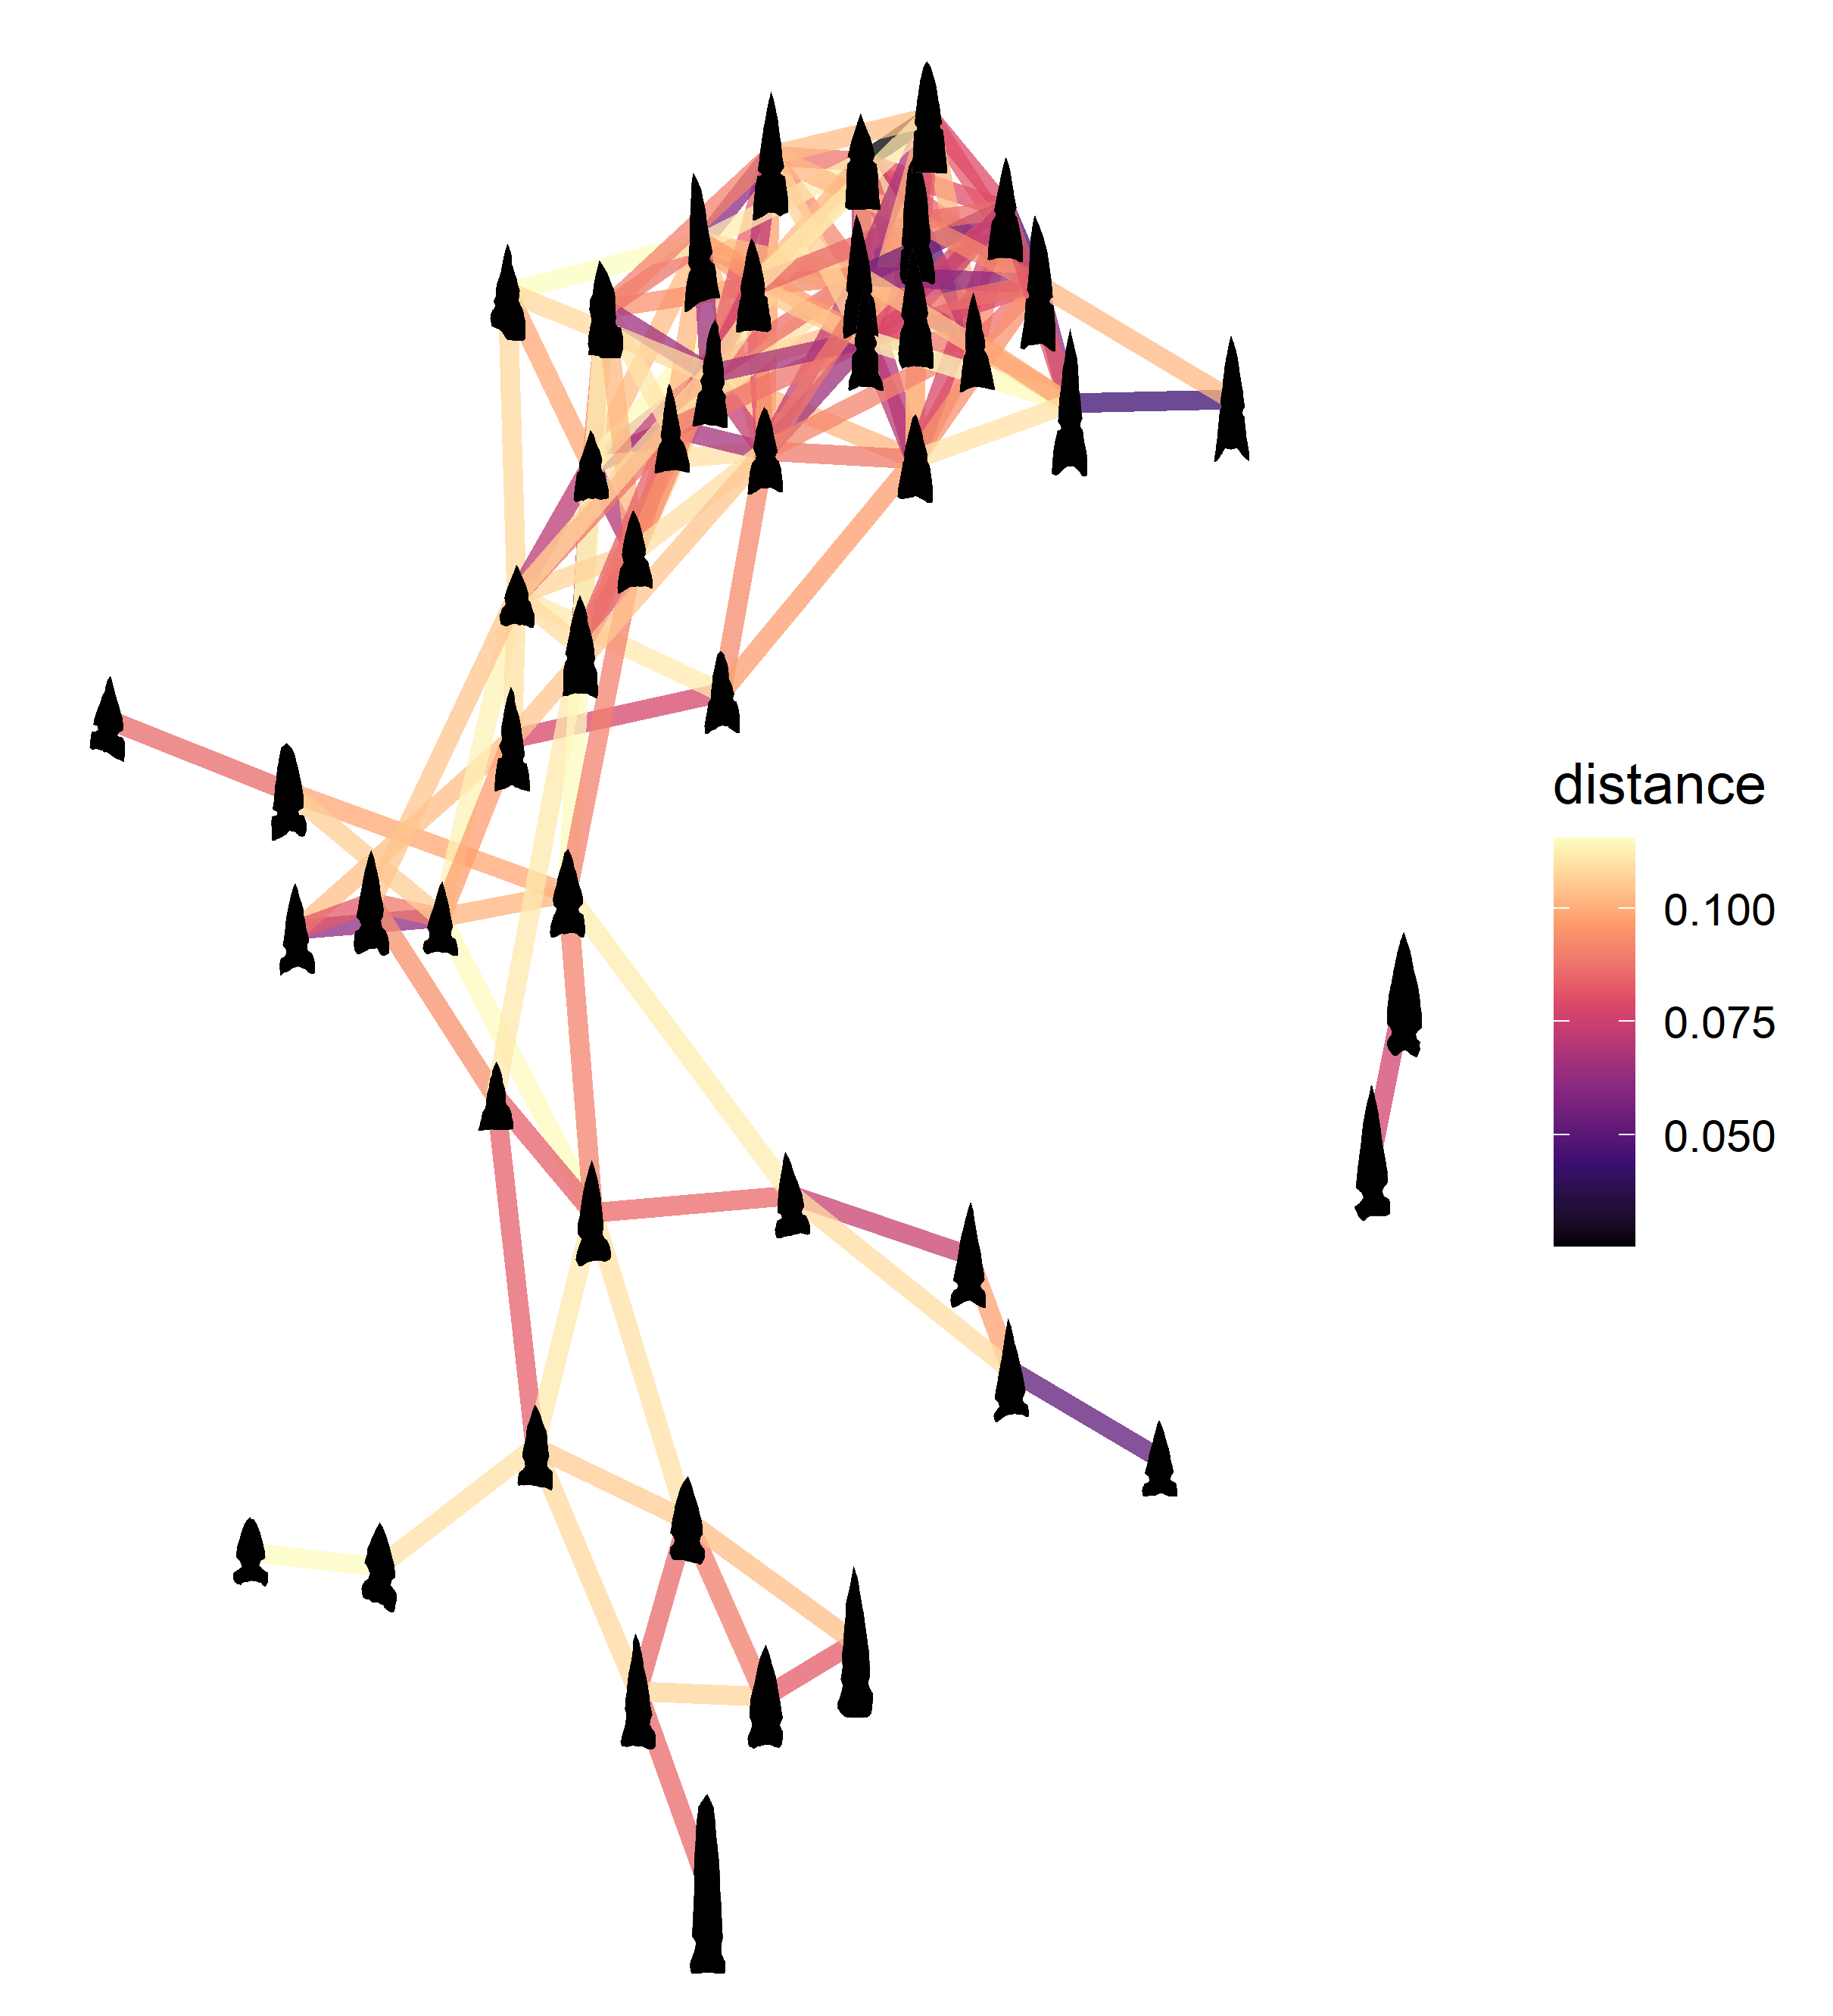
\includegraphics[width=1\linewidth]{figures/TontoSideDistanceNetwork} \caption{Network graph displaying side-notched points from Tonto Basin as nodes with ties showing the morphometric distance between points. Darker colors represent stronger ties. Note that only the strongest 10\% of ties are shown. From Bischoff (2022: Figure 14).}\label{fig:TontoSideDistanceNetwork}
\end{figure}

\begin{figure}
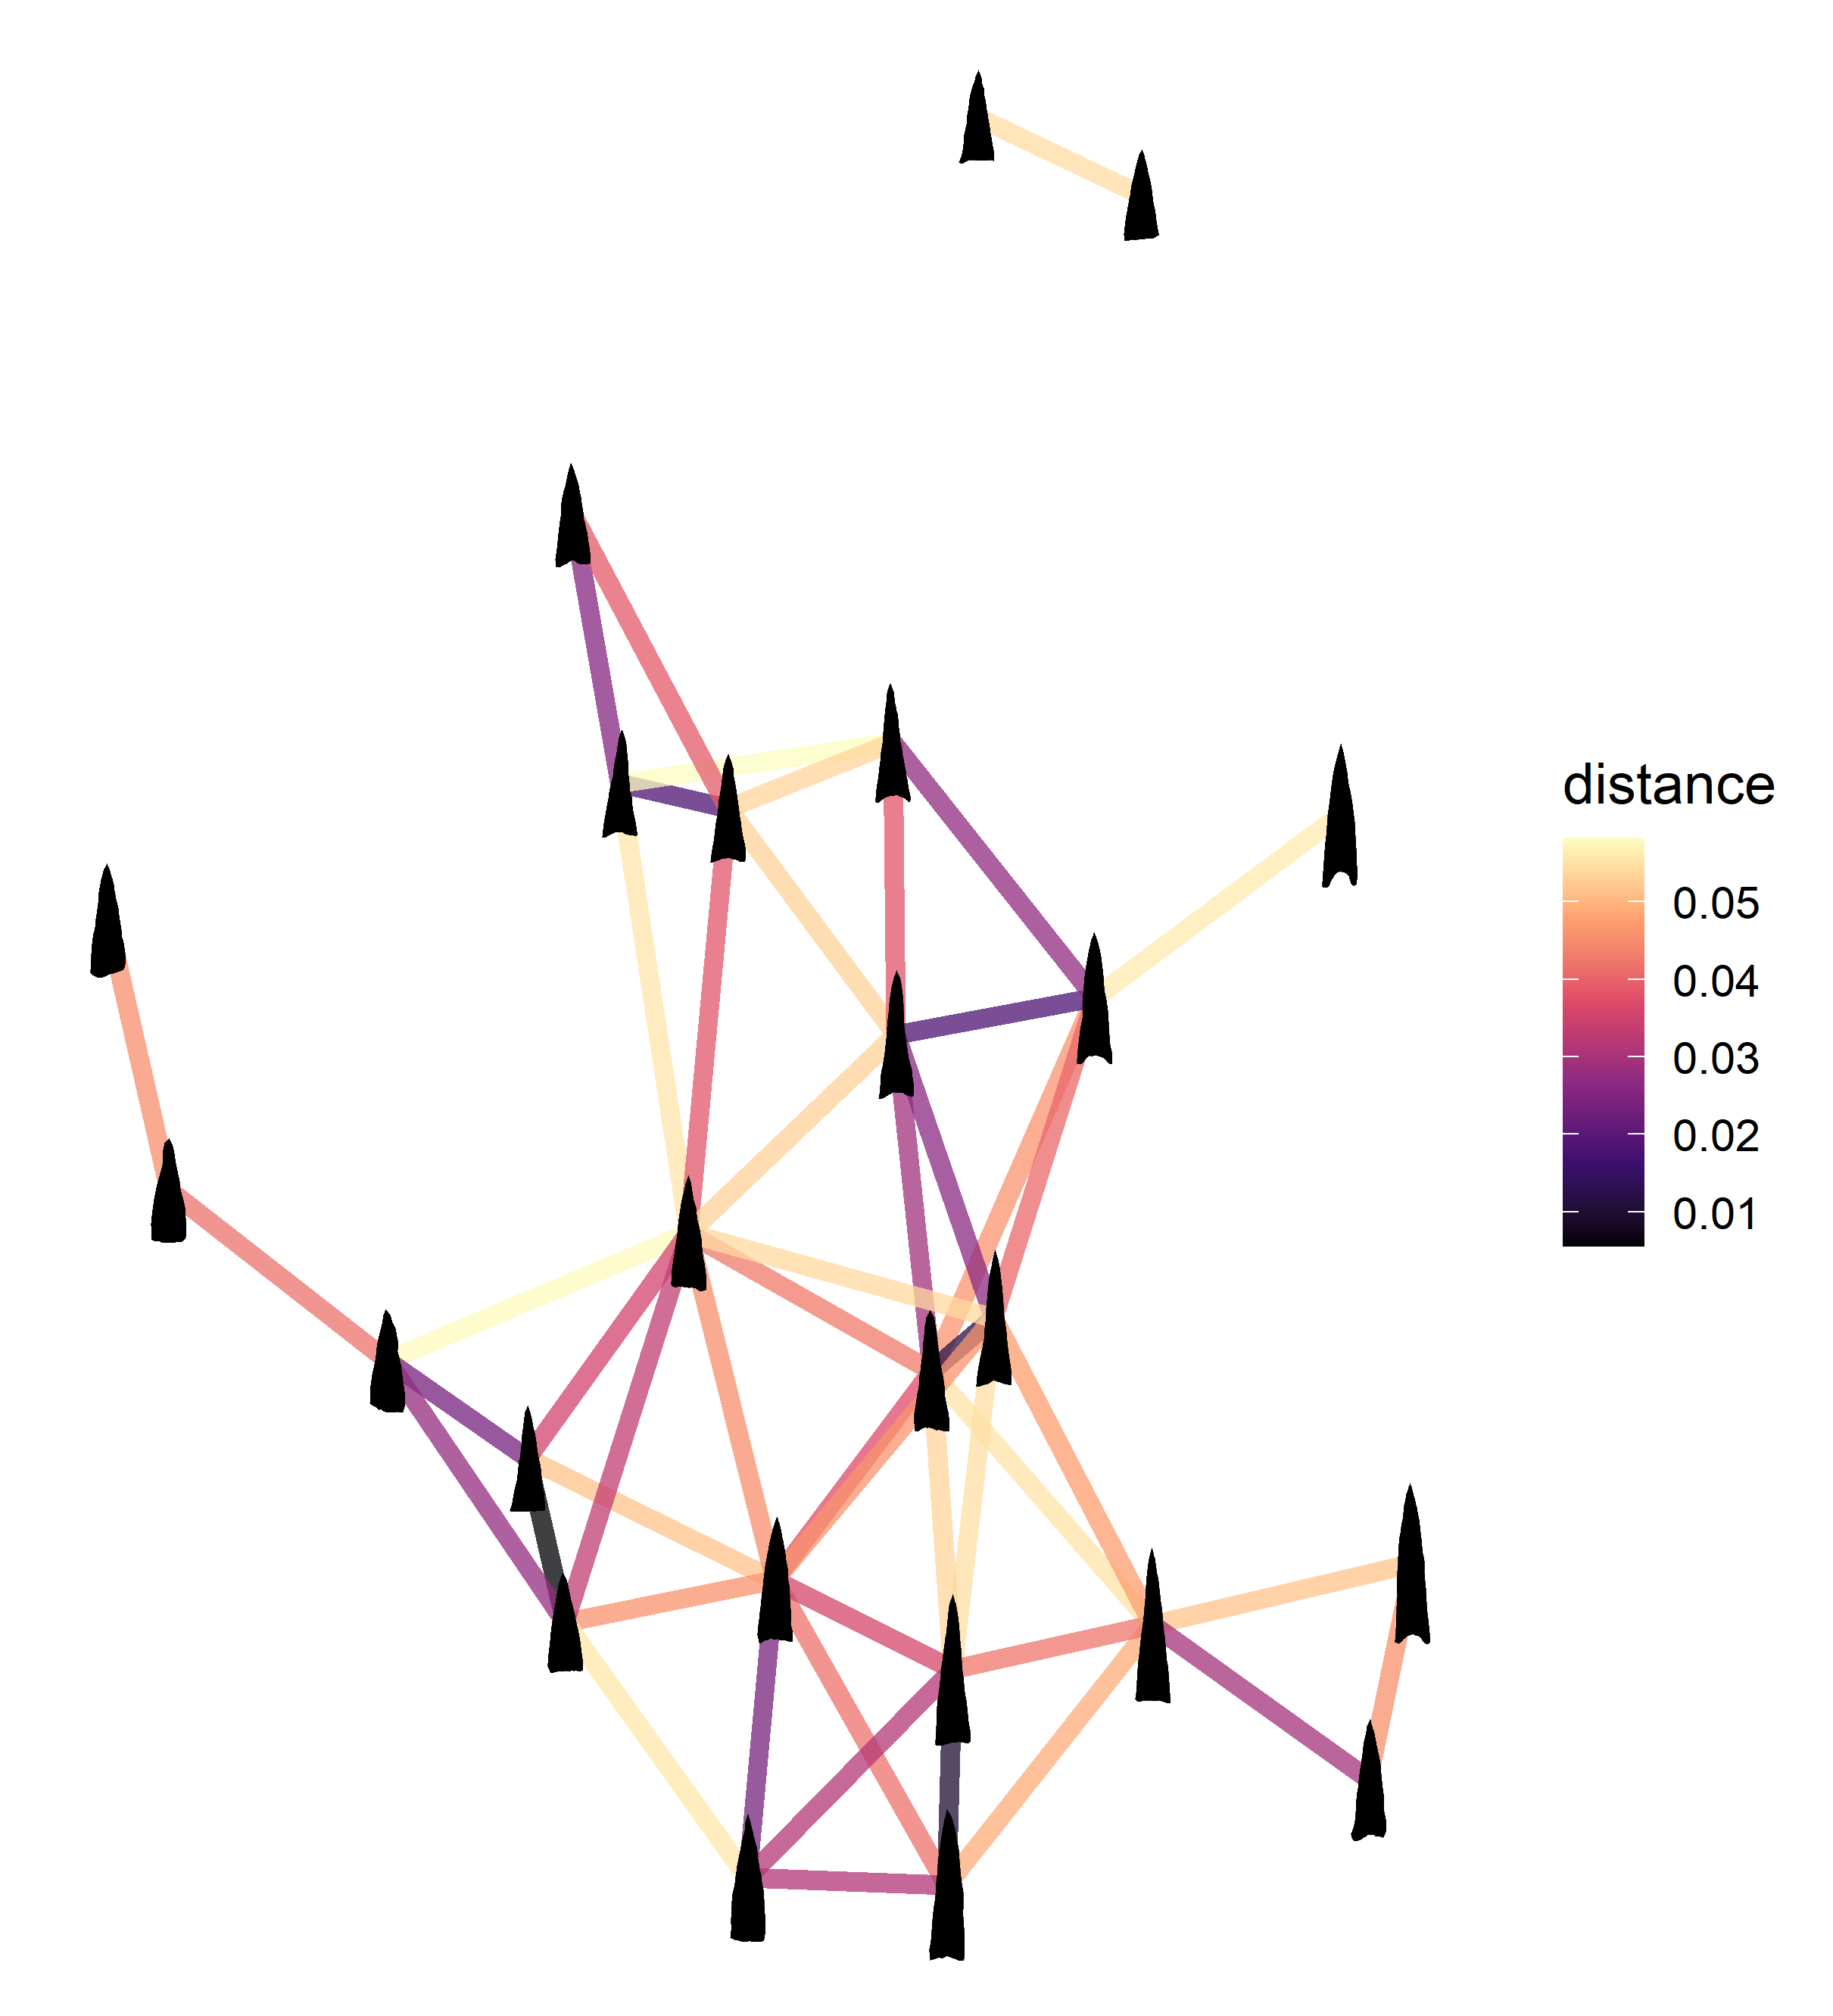
\includegraphics[width=1\linewidth]{figures/TontoTriangularDistanceNetwork} \caption{Network graph displaying triangular points from Tonto Basin as nodes with ties showing the morphometric distance between points. Darker colors represent stronger ties. Note that only the strongest 10\% of ties are shown. From Bischoff (2022: Figure 15).}\label{fig:TontoTriangularDistanceNetwork}
\end{figure}

\hypertarget{results}{%
\section*{Results}\label{results}}
\addcontentsline{toc}{section}{Results}

A major benefit of network analysis is the visual exploration of the
network. The results of the network analysis are provided partially to
address the major questions of this paper--the correlations between
types of material culture and their potential causes--and partially as a
visual exploration with corresponding evidence from network metrics.

Figure 4 shows the networks with the top five strongest ties between
each node. This number of ties represents the fewest ties that connects
all nodes in the spatial network. Fewer ties leaves the Cline Mesa sites
disconnected from the rest of the network. Bass Point Mound forms a
crucial bridge between the Cline Mesa sites and the rest of the network.
Because the network is not complete, one cannot argue that there were
not other sites between Cline Mesa and the Schoolhouse Mesa sites, but
it still represents an intermediary location. Its geographic position
overlooking the confluence of the Salt River and Tonto Creek would make
an ideal meeting place for parties coming down from the Tonto Creek arm
of what is now Roosevelt Lake or coming up from the Salt River arm. The
Rock Island area consists of a single site, Bass Point Mound (a platform
mound), although it was not heavily excavated. If spatial distance was
an important factor in social interaction, then we would expect Bass
Point Mound to consistently be a highly central node due to its central
location. Table 2 shows the multilayer eigenvector centrality for points
and ceramics only. Bass Point Mound has the highest multilayer network
centrality with 0.95 (p = 0.87). Figure 5 provides the eigenvector data
by type of network. Bass Point Mound has low centrality in the
architectural network and the networks that do not connect the spatial
components (three and four closest connections), which gives it a lower
spatial centrality as well. The ceramic and point networks provide
strong evidence that Bass Point Mound's spatial location was
advantageous for forming connections between the sites in this study.

\begin{figure}
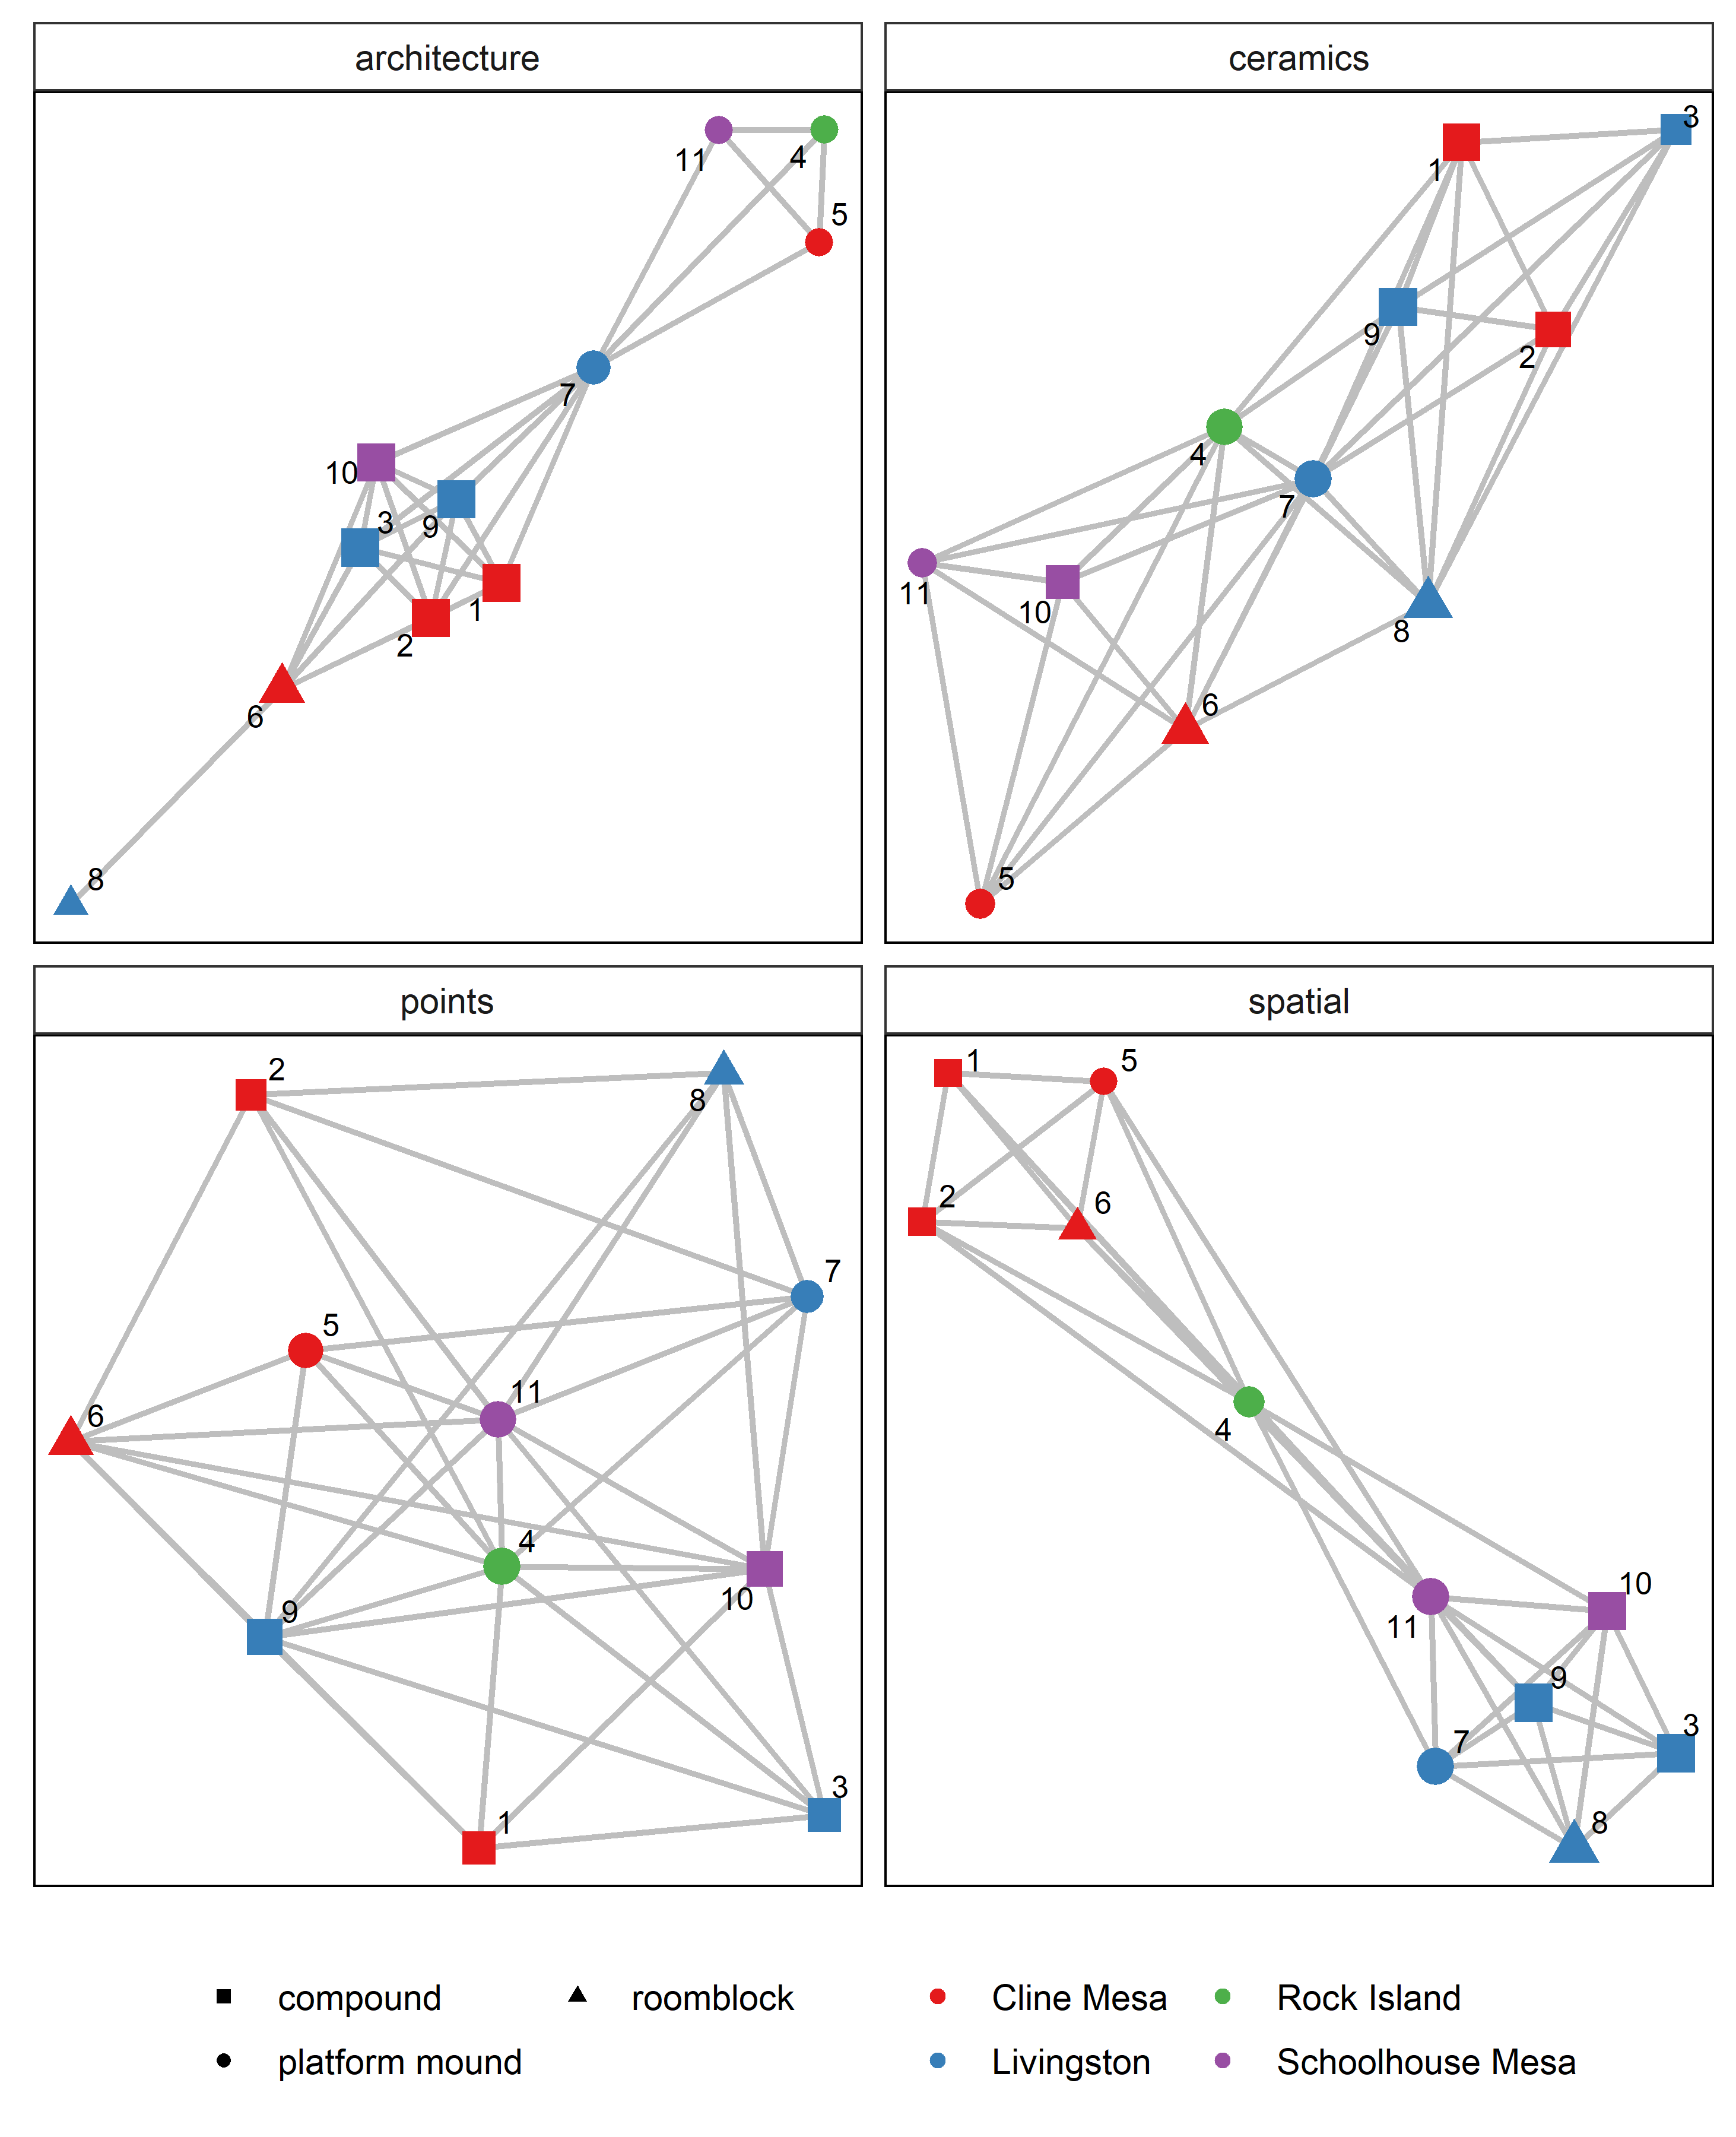
\includegraphics[width=1\linewidth]{figures/TontoNetworksMultiNet} \caption{Graphs showing the networks used in this analsyis. Each network is displayed with the five strongest ties between each node. Legend: 1: AZ U:3:128 (ASM); 2: AZ U:4:032 (ASM); 3: AZ V:5:119 (ASM); 4: Bass Point Mound; 5: Cline Terrace Mound, Monster Ruin; 6: Indian Point Complex; 7: Pinto Point Mound; 8: Saguaro Muerto; 9: Sand Dune Site; 10: Schoolhouse Point Mesa Complex; 11: Schoolhouse Point Mound}\label{fig:TontoNetworksMultiNet}
\end{figure}

\begin{table}

\caption{\label{tab:meanEigen}Multilayer Eigenvector Centrality for Ceramics and Points}
\centering
\begin{tabular}[t]{lr}
\toprule
Site & Centrality\\
\midrule
Bass Point Mound & 0.95\\
Sand Dune Site & 0.84\\
Pinto Point Mound & 0.76\\
Indian Point Complex & 0.65\\
AZ U:3:128 (ASM) & 0.64\\
\addlinespace
Schoolhouse Point Mesa Complex & 0.59\\
Schoolhouse Point Mound & 0.55\\
Cline Terrace Mound, Monster Ruin & 0.50\\
Saguaro Muerto & 0.49\\
AZ U:4:032 (ASM) & 0.46\\
\addlinespace
AZ V:5:119 (ASM) & 0.30\\
\bottomrule
\end{tabular}
\end{table}

Visual inspection of the network graphs provides several other
observations. One is that the four geographic areas represented do not
form strong components in the non-spatial networks like they do in the
spatial network. The architecture is thoroughly mixed, and the ceramics
and points form single component networks. The formation of single
components--rather than distinct sections of the graph--is typical of
artifact similarity networks. The Livingston sites exhibit the most
clustering in the ceramic network, although some of the connections go
through Cline Mesa sites, which are as geographically distant as
possible for these sites. The Schoolhouse Mesa sites always group
together in the ceramic and point networks, as do the Livingston
compound sites and separately the Livingston roomblock and platform
mound. The Cline Mesa sites exhibit more variability.

\begin{figure}
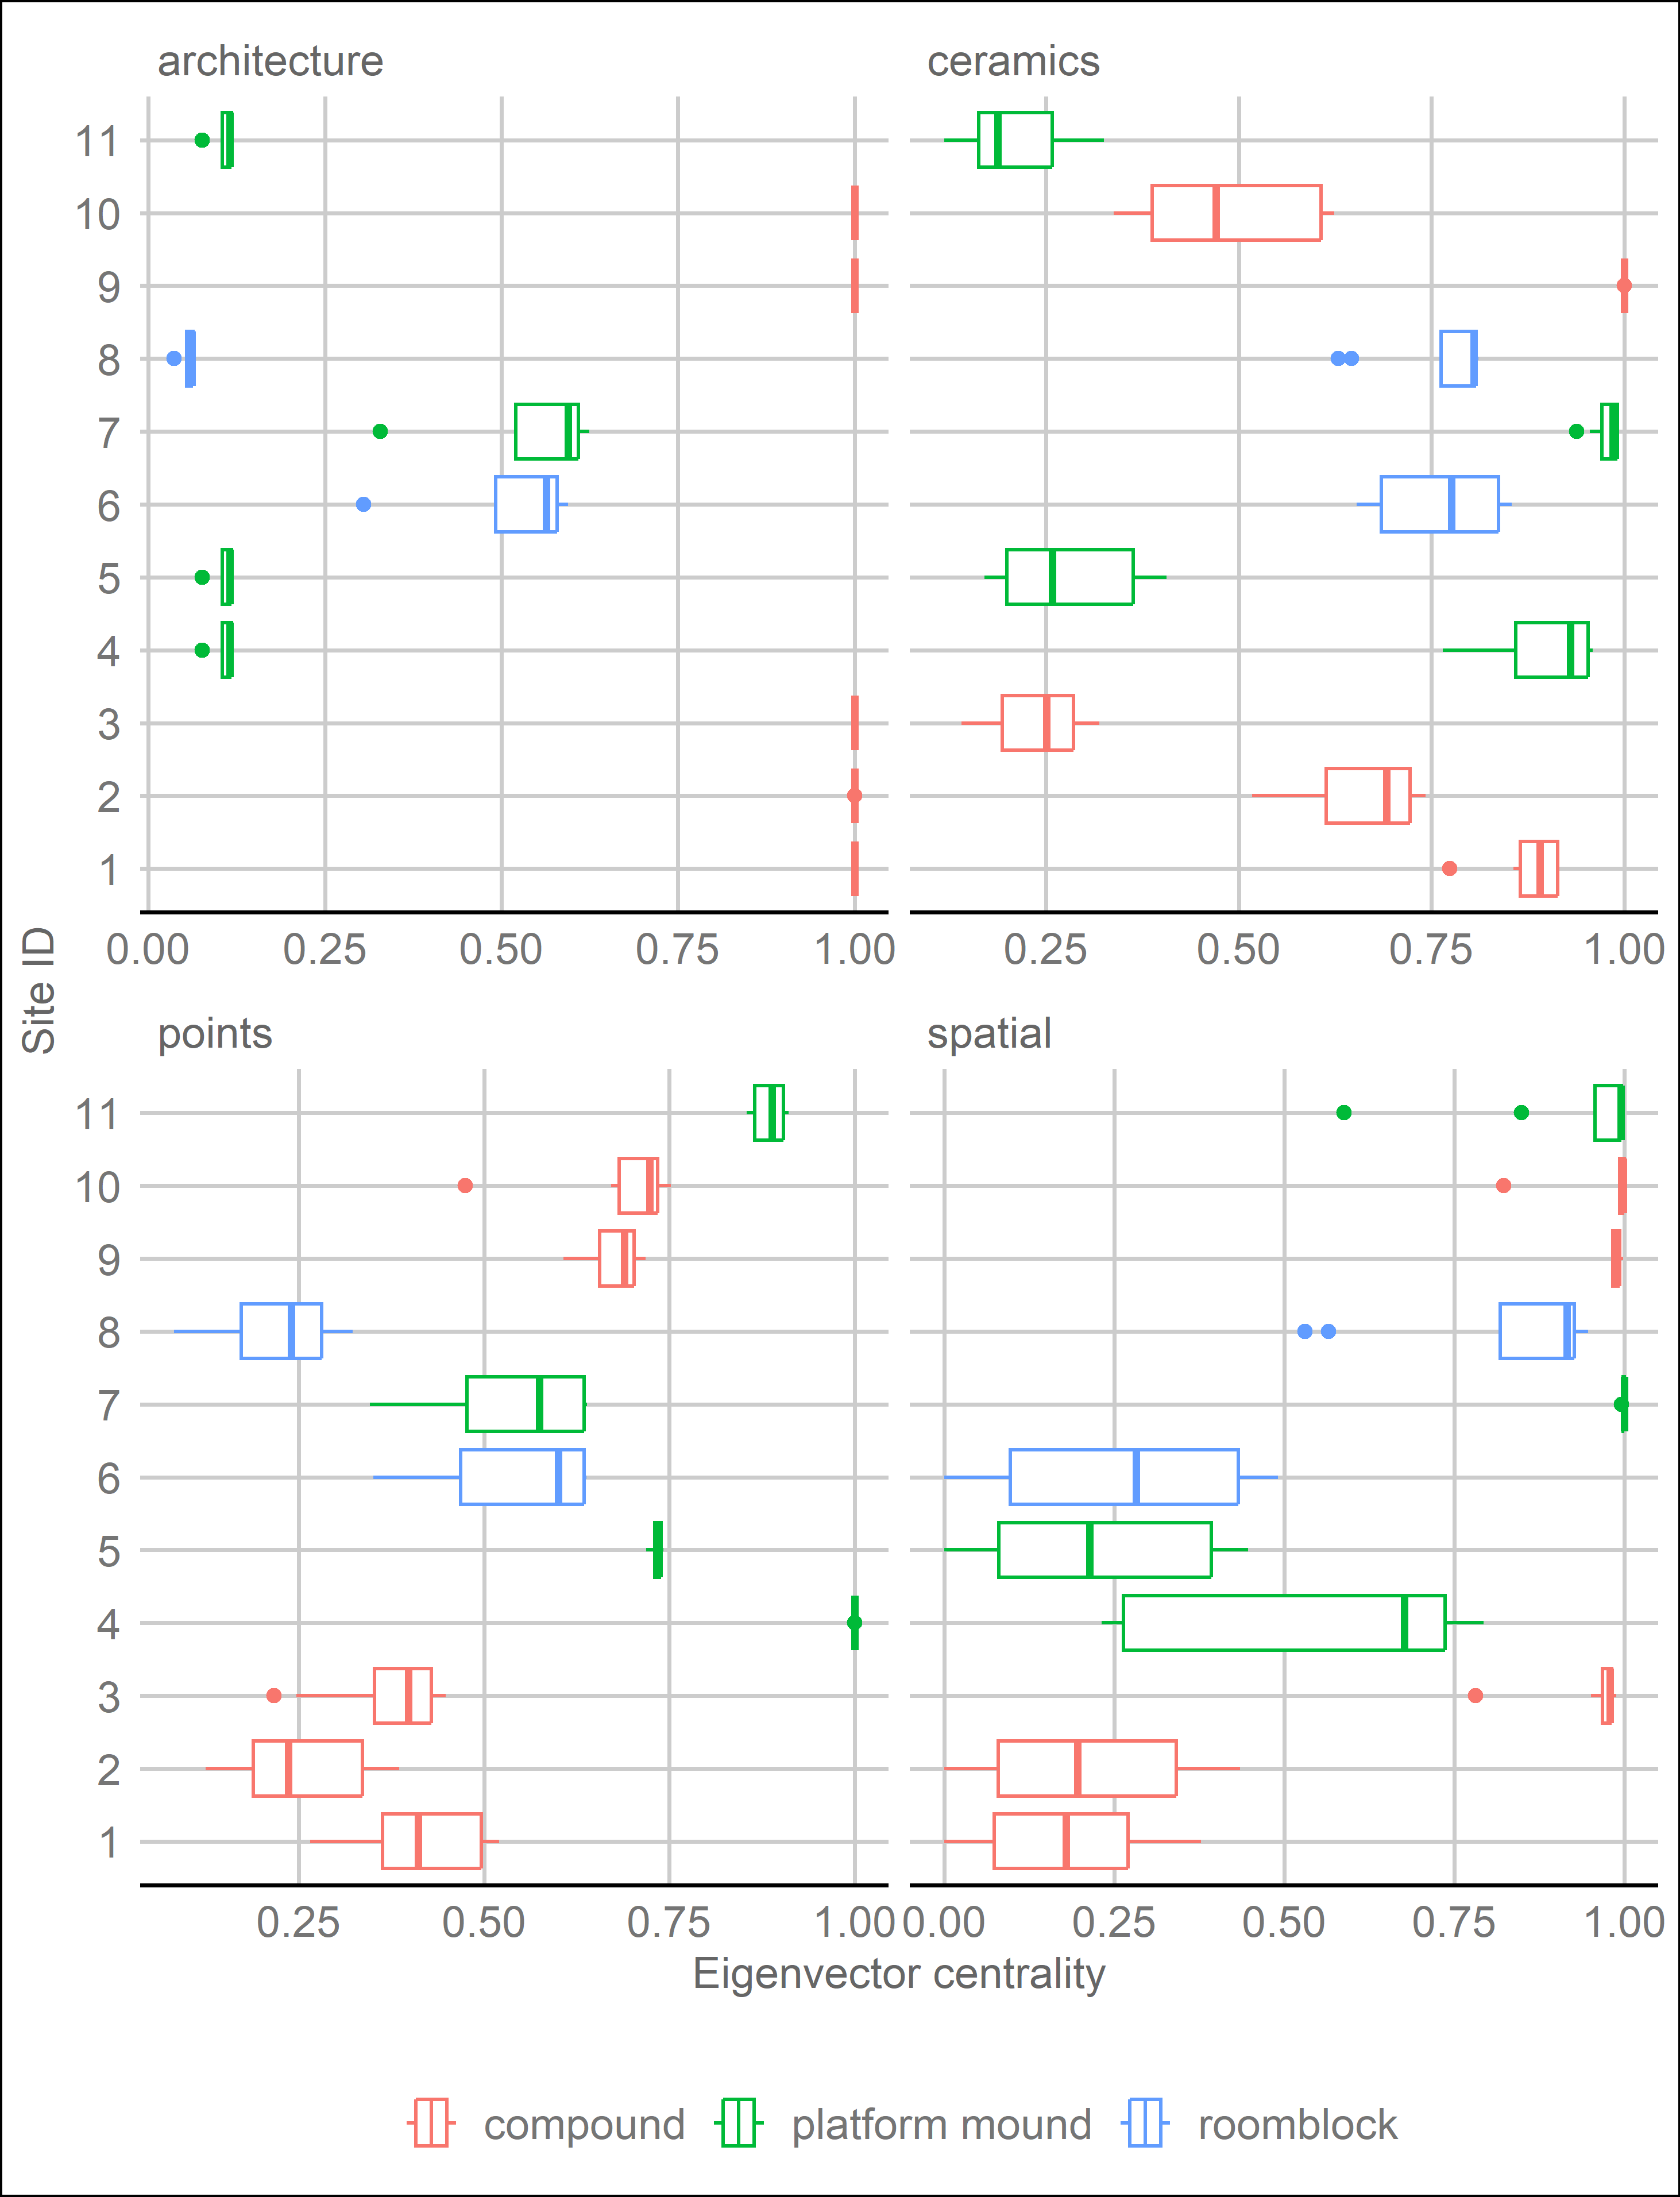
\includegraphics[width=1\linewidth]{figures/TontoNetworksEigenvector} \caption{Boxplots showing the eigenvector centrality for each network. Values were calculated using networks created using between 3 to 10 of the strongest ranking ties. Legend: 1: AZ U:3:128 (ASM); 2: AZ U:4:032 (ASM); 3: AZ V:5:119 (ASM); 4: Bass Point Mound; 5: Cline Terrace Mound, Monster Ruin; 6: Indian Point Complex; 7: Pinto Point Mound; 8: Saguaro Muerto; 9: Sand Dune Site; 10: Schoolhouse Point Mesa Complex; 11: Schoolhouse Point Mound.}\label{fig:TontoNetworksEigenvector}
\end{figure}

Another observation from the visual inspection of these networks is that
there is some clustering due to architecture in the ceramic and point
networks. Four of the five compound-only sites cluster at one end of the
ceramic network, and a different mix of four out of five cluster
together at one end of the projectile point network. The platform mounds
are split in the ceramic network, but all cluster together in the
projectile point network. Table 3 shows the mean eigenvector centrality
vectors for the ceramic and point networks by type of architecture.
Surprisingly the platform mounds are the least central, on average, for
the ceramic network, but they are the most central for the projectile
point network. The roomblocks, on the hand, are the most central for the
ceramic network and by far the least central in the projectile point
network. They take a larger drop in centrality in the projectile point
network than the platform mound sites do in the ceramic network. It is
expected that roomblocks have high centrality in the ceramic network,
but not that platform mounds should have the lowest centrality. Clearly,
centrality in the projectile point network does not equal centrality in
the ceramic network.

\begin{table}

\caption{\label{tab:meanEigenVals}Mean Eigenvalues for Ceramic and Point Networks by Type of Architecture}
\centering
\begin{tabular}[t]{lrrr}
\toprule
Architecture & ceramics & points & mean\\
\midrule
platform mound & 0.59 & 0.79 & 0.69\\
roomblock & 0.76 & 0.38 & 0.57\\
compound & 0.65 & 0.48 & 0.56\\
\bottomrule
\end{tabular}
\end{table}

The visual analysis, combined with the eigenvector centrality, indicated
some spatial and architectural correlation. The multilayer Pearson
correlation provides a more direct way to compare these layers, as shown
in figure 6. This analysis provides a clear contrast between layers.
None of the results, on average, showed a negative correlation--meaning
that ties existed in one network where ties did not exist in the other
network. Only one comparison had a strong correlation--the point and
spatial networks were strongly correlated (\textbf{x} = 0.63; p = 0.98).
The visual inspection and centrality analysis provided some indication
of this, but the multilayer network comparison provides strong
verification. All other layer comparisons had an approximately
equivalent, positive correlation, but with only a weak strength. The one
exception was architecture and points where the correlation was
approximately zero. The visual inspection and eigenvector analysis
demonstrated some interesting interactions with architecture in the
network, but the overall correlation demonstrates that architecture
cannot be used to predict the presence or absence of network ties in the
projectile point network.

\begin{figure}
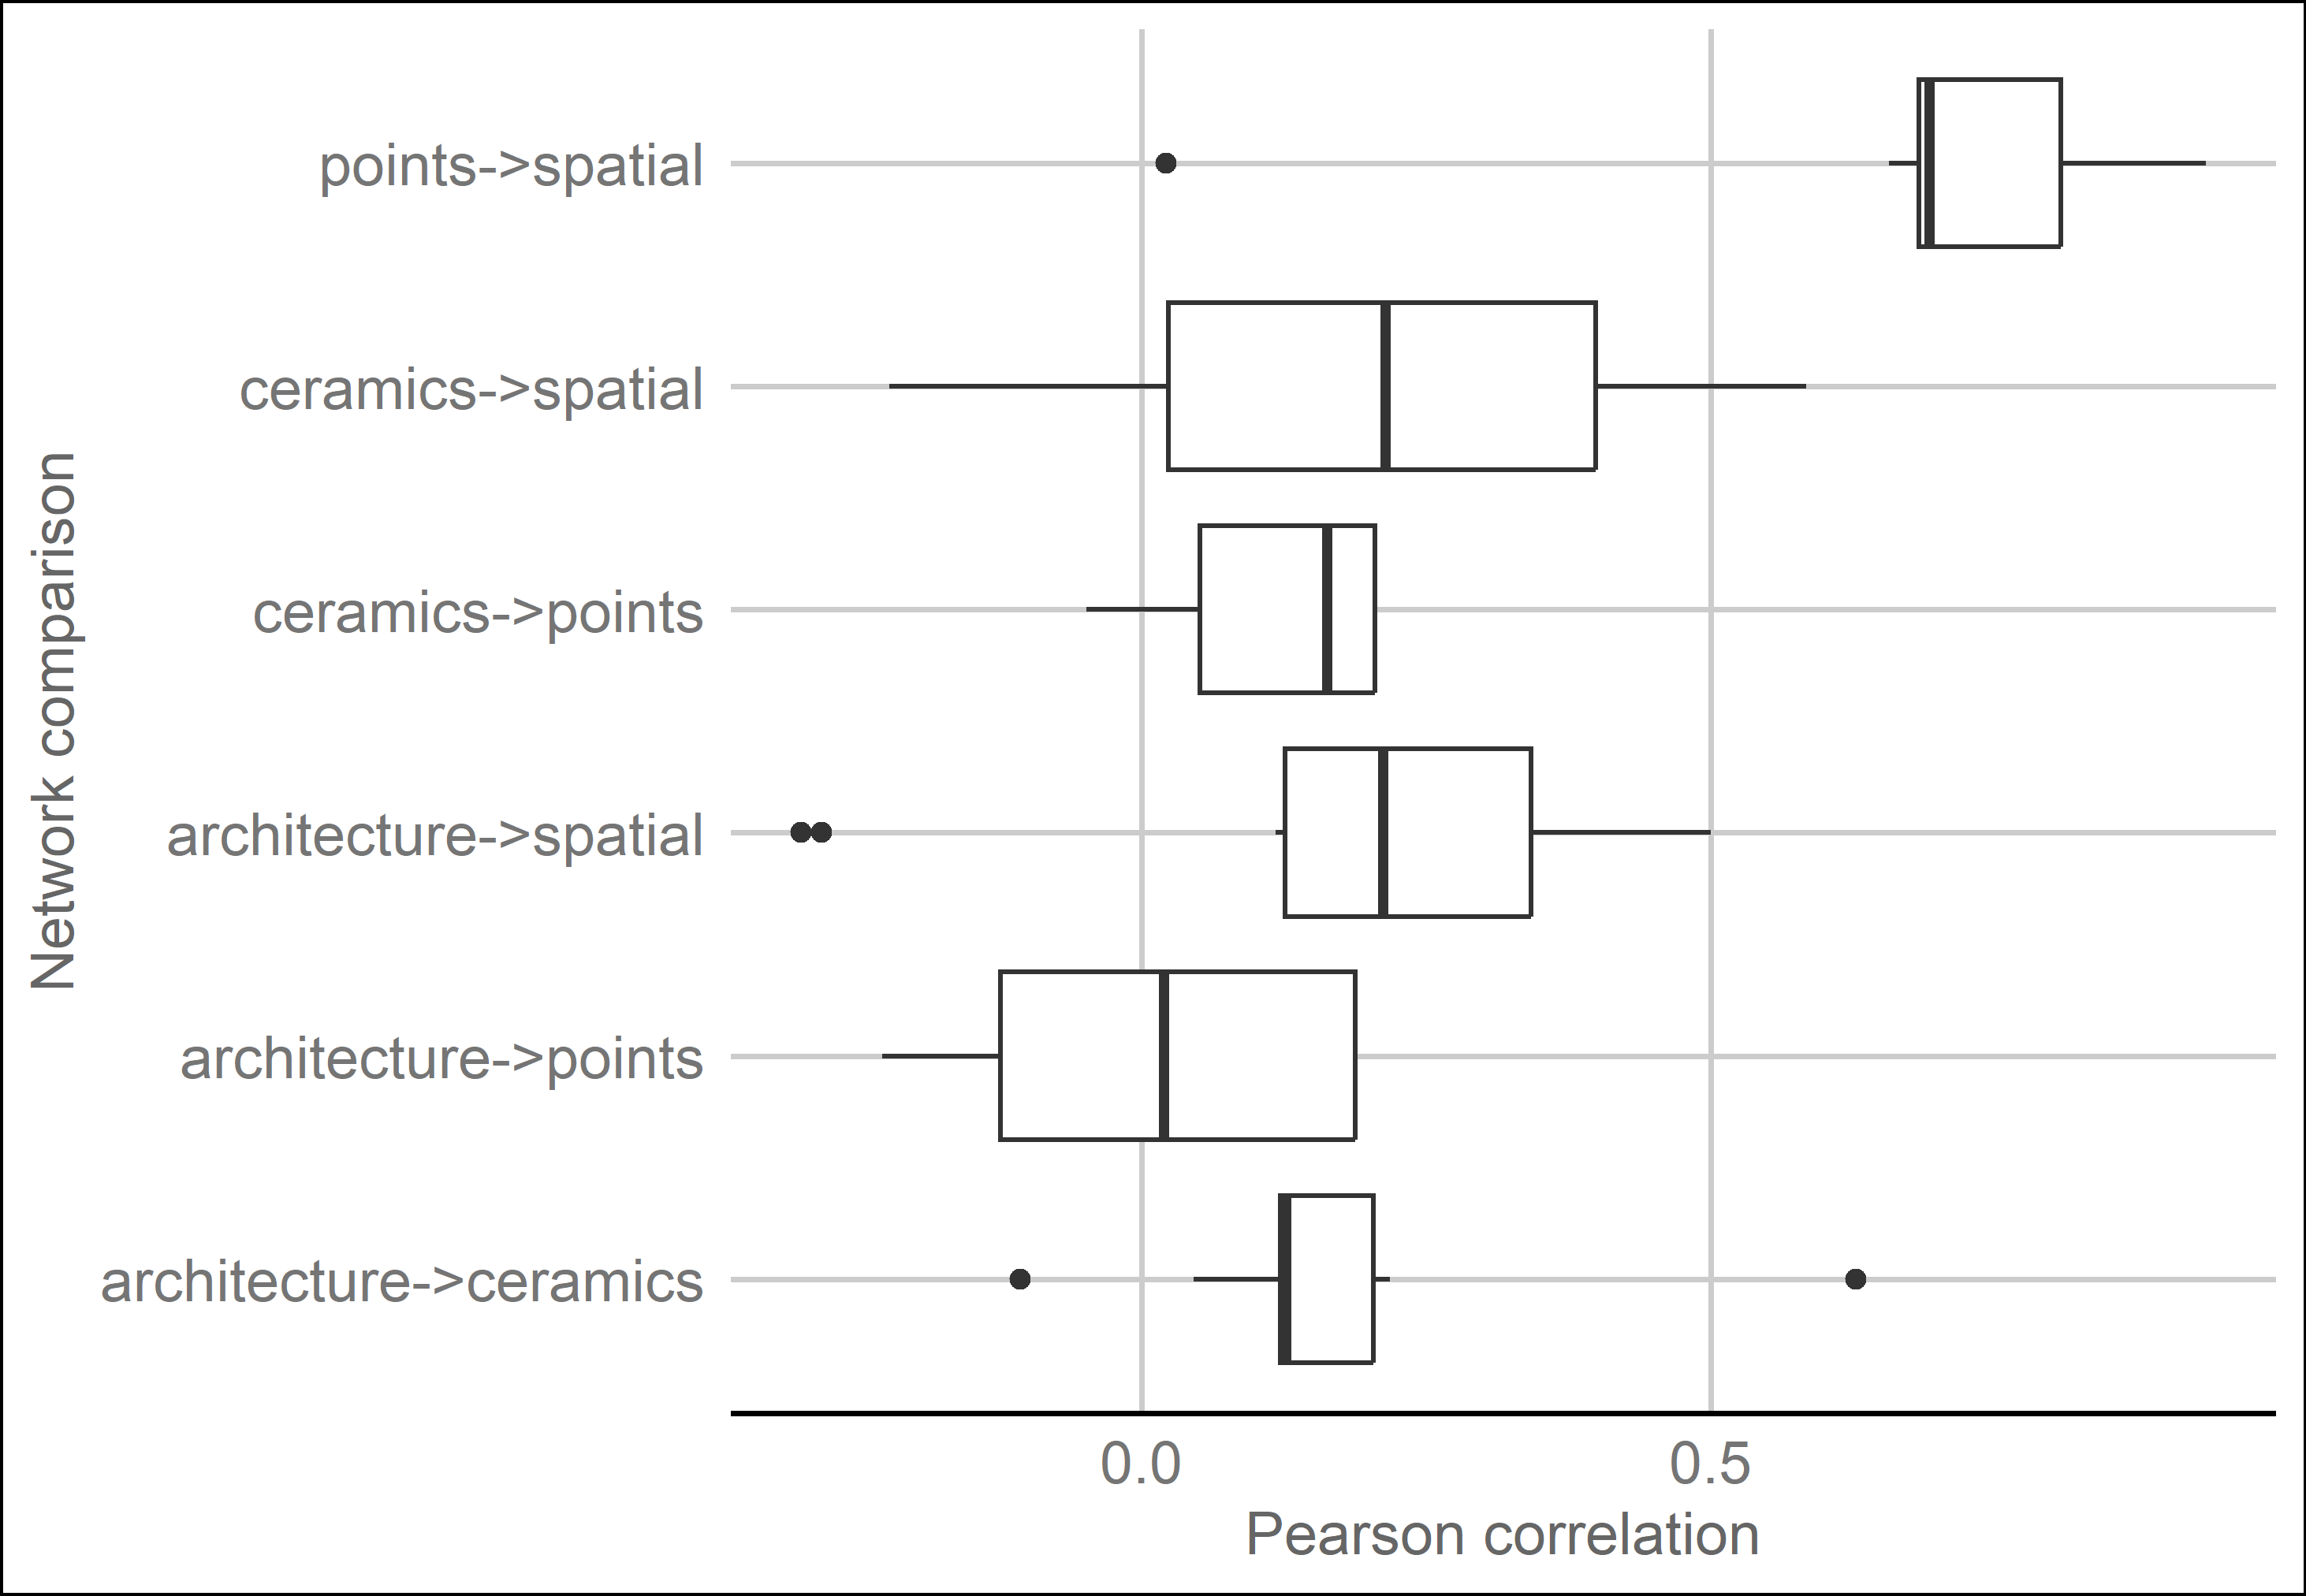
\includegraphics[width=1\linewidth]{figures/TontoNetworksCorrelation} \caption{Boxplots showing the Pearson correlation between each network. Values were calculated using networks created from 3 to 10 of the strongest ranking ties.}\label{fig:TontoNetworksCorrelation}
\end{figure}

\hypertarget{discusssion}{%
\section*{Discusssion}\label{discusssion}}
\addcontentsline{toc}{section}{Discusssion}

This analysis has three main findings regarding networks in Tonto Basin:
(1) that point networks correlate with space; (2) that roomblock sites
are highly central in the ceramic network and have low centrality in the
point network; and (3) that ceramic and point networks are significantly
different from each other. In terms of the null hypotheses stated in the
introduction, only one of the networks exhibited strong spatial
correlation and while all but one pairing (architecture and points)
exhibited some positive correlation, all of the correlations except the
points and space were weak. Given these network results, how might they
be interpreted in terms of social behavior?

Exchange would be a primary driver in these network dynamics, and clear
evidence exists for exchange of several types of material culture. Trade
within the basin does not appear to have been dominated by any one group
and may have been competitive in nature \citep[p.~127-128]{Rice1998-cu}.
Ceramic exchange certainly occurred at a regional level, but even local
ceramics were circulated within the basin
\citep{Heidke2000-nr, Miksa1995-qw, Stark1992-vu}, possibly in return
for food \citep[p.290-291]{Clark2004-uw}. Projectile points (either as
part of the arrow or separately) may have also been commonly exchanged.
There are several examples of the exchange of bows and arrows
ethnographically throughout the world
\citep[e.g.,][]{Mauss1966-nm, Nishiaki2013-lc, Wiessner1983-ei}, in
North America generally \citep[e.g.,][]{Hoffman1896-xl, Radin1923-gf},
and in the Southwest specifically
\citep[e.g.,][]{Beaglehole1936-ul, Dittert1959-rz, Fewkes1898-oj, griffen1969a, Parsons1939-xg, Simpson1953-ob}.
Besides Watt's study of knappers, Sliva's
\citeyearpar[p.~539]{Sliva2002-oz} analysis of sites from the Roosevelt
Community Development Study suggests craft specialization in projectile
point production. Mortuary offerings were possibly the intended function
for many points \citep[p.~543]{Sliva2002-oz}, which may have spurred the
increased craft specialization. Shell and stone jewelry, among other
artifacts were also produced and exchanged within the basin. A potential
loci for exchange are the platform mound sites. The purpose of these
sites is still debated, but many argue that they served an integrative
function
\citetext{\citealp[e.g.,][]{Abbott2006-fg}; \citealp{Adler1990-ws}; \citealp{Clark2004-uw}; \citealp{Craig1995-qo}; \citealp[p.~112-165]{Craig1994-bg}; \citealp[p.~439]{Doelle1995-qd}}.
If platform mounds were places where exchange between communities
regularly took place, then we would expect platform mounds to have
higher centrality. Centrality varied among the platform mounds, but on
average, platform mounds did have the highest centrality.

As discussed previously, cultural differences were expected between the
Tonto Creek and Salt River arms of Roosevelt Lake. This was due in part
to differences in long-distance ceramic exchange and obsidian sourcing
\citep{Lyons2013-ya, Simon2001-am}. This analysis did not use obsidian
or focus on non-local ceramics and therefore did not capture differences
based on these factors. There was some expectation that more separation
in the material networks would be apparent between the Cline Mesa sites
in the Tonto Creek arm and the other sites (minus Bass Point Mound that
lies at the confluence). This was not born out in the visual inspection
of the analysis with significant mixing of the areas in the network.
There were, however, indications that spatial distance was an important
factor. Spatial distance would align with the proposed differences in
the Tonto Creek and Salt River arms of the lake. The only strong
correlation between networks was the point and spatial network, which
indicates that being near another site is a good indication of the shape
of a projectile point. There was however, little correlation overall
between ceramics and spatial distance.

There is a potential chain of association between immigrants and
roomblocks, roomblocks or locations with roomblocks as centers of Salado
production, and Salado pottery as a widespread phenomenon that provides
an expectation for roomblock sites to be central to pottery networks.
While this association is circumstantial and not expected to be uniform
across the Hohokam region, roomblocks did have the highest centrality in
the ceramic networks. Another reason for the high centrality of
roomblock sites is that they lacked access to adequate farmland and had
to trade pottery for food \citep[p.~291]{Clark2004-uw}. This second
explanation may help explain why roomblock sites had low centrality in
the point networks, presuming that points were not exchanged for food.
It is beyond this simple analysis to determine the precise reasons, but
it is clear that roomblock sites were important for ceramic circulation
in Tonto Basin. On the other hand, sites with roomblocks had the lowest
centrality in the point networks. This suggests that the influence the
occupants of roomblock sites had in pottery networks may not have
extended to other spheres of interaction.

As discussed previously, my simplistic model of interaction in Tonto
Basin assumes that the ceramic network represents categorical
identification among women. Recall also that I expected architecture to
represent categorical identity. Thus, the correlation between
architecture and ceramics, at least as represented by roomblocks, is an
expected find and good corroborating evidence that these types of
material culture represent markers of identity demonstrating belonging
to a particular social group.

The point networks were expected to represent relational identification
among men, at least in this case study. Because relational
identification is related to frequent interaction, spatial distance is a
crucial component. It is much harder to interact with someone when they
are far away. Thus, the correlation between the point and spatial
networks also makes theoretical sense.

Perhaps the reason roomblocks were more central to the ceramic network
is because immigrants to the basin had less access to farmland and had
to make pottery to get food, as mentioned. This would explain higher
centrality for roomblocks and lower centrality for point networks. It
does not explain the remaining differences between point and ceramic
networks. Projectile points at least were highly gendered, and ceramics
probably were as well. The evidence presented here demonstrates that
ceramic and point networks vary significantly, and I believe gender
likely played an important role.

\hypertarget{conclusion}{%
\section*{Conclusion}\label{conclusion}}
\addcontentsline{toc}{section}{Conclusion}

This is one of the first archaeological applications of multilayer
network analysis to consider multiple types of material culture. This is
advantageous for studying how types of material culture do or do not
co-vary, which aids interpretations of the social interactions that
created these patterns. This analysis used architectural, ceramic,
projectile point, and spatial data from 11 sites in Tonto Basin. The
data come primarily from occupations between AD 1275 and 1325. A network
was created for each type of data and combined into a multilayer
network. Visual network analysis, eigenvector centrality, and multilayer
network Pearson correlation were used to study and compare the networks.
The findings indicate that the projectile point network was strongly
correlated with the spatial network--indicating that sites near each
other were more likely to have similar projectile points. Furthermore,
sites with roomblocks indicative of immigrants from the north and east
of Tonto Basin were, on average, the most highly central sites in the
ceramic network; however, they were the least central in the point
network. Immigrants may have relied on pottery production to integrate
with the local networks, but this relationship did not hold for
projectile points. Finally, the results demonstrate major differences
between the ceramic and point networks. This findings has major
implications for network studies, because many rely on only a single
artifact type. If different types of material culture do not co-vary
regularly, then that indicates archaeologists must do more to include
other types of material culture to better understand the complex social
networks that existed in the past. Furthermore, projectile points and
ceramics have strong associations with gender. Differences in the
ceramic and point networks suggest differences existed between the
social networks of each gender.

This analysis uses a handful of sites from Tonto Basin. Much more data
exists and the results discussed here would be greatly strengthened by
including more sites and data. What would be perhaps even more useful
would be to include sourced obsidian and ceramics. Networks created from
artifacts where the origin is known can be used to more strongly infer
various types of social interaction. This type of multilayer analysis
would also be useful to conduct in other regions. It would be
particularly useful for comparative studies to know in what
circumstances different types of material culture do or do not co-vary.

\hypertarget{acknowledgements}{%
\section*{Acknowledgements}\label{acknowledgements}}
\addcontentsline{toc}{section}{Acknowledgements}

Josh Watts, Matt Peeples, Melissa Powell, Chris Caseldine, and several
volunteers assisted with this research. Chris Caseldine's comments
greatly improved this paper. All mistakes are my own. The many
individuals who contributed to the Roosevelt Platform Mound Study also
deserve recognition.

\hypertarget{disclosure-statement}{%
\section*{Disclosure Statement}\label{disclosure-statement}}
\addcontentsline{toc}{section}{Disclosure Statement}

The author declares no conflicts of interest.

\bibliographystyle{tfcad}
\bibliography{references2.bib}





\end{document}
